%% History:
% Pavel Tvrdik (26.12.2004)
%  + initial version for PhD Report
%
% Daniel Sykora (27.01.2005)
%
% Michal Valenta (3.12.2008)
% rada zmen ve formatovani (diky M. Duškovi, J. Holubovi a J. Žďárkovi)
% sjednoceni zdrojoveho kodu pro anglickou, ceskou, bakalarskou a diplomovou praci

% One-page layout: (proof-)reading on display
%%%% \documentclass[11pt,oneside,a4paper]{book}
% Two-page layout: final printing
\documentclass[11pt,twoside,a4paper]{book}   
%=-=-=-=-=-=-=-=-=-=-=-=--=%
% The user of this template may find useful to have an alternative to these 
% officially suggested packages:
\usepackage{color}
\usepackage[czech, slovak, english]{babel}
\usepackage[T1]{fontenc} % pouzije EC fonty 
% pripadne pisete-li cesky, pak lze zkusit take:
% \usepackage[OT1]{fontenc} 
\usepackage[utf8]{inputenc}
\usepackage{enumerate}
\usepackage{multirow}
\usepackage{capt-of} %captionof
%=-=-=-=-=-=-=-=-=-=-=-=--=%
% In case of problems with PDF fonts, one may try to uncomment this line:
%\usepackage{lmodern}
%=-=-=-=-=-=-=-=-=-=-=-=--=%
%=-=-=-=-=-=-=-=-=-=-=-=--=%
% Depending on your particular TeX distribution and version of conversion tools 
% (dvips/dvipdf/ps2pdf), some (advanced | desperate) users may prefer to use 
% different settings.
% Please uncomment the following style and use your CSLaTeX (cslatex/pdfcslatex) 
% to process your work. Note however, this file is in UTF-8 and a conversion to 
% your native encoding may be required. Some settings below depend on babel 
% macros and should also be modified. See \selectlanguage \iflanguage.
%\usepackage{czech}  %%%%%\usepackage[T1]{czech} %%%%[IL2] [T1] [OT1]
%=-=-=-=-=-=-=-=-=-=-=-=--=%

%%%%%%%%%%%%%%%%%%%%%%%%%%%%%%%%%%%%%%%
% Styles required in your work follow %
%%%%%%%%%%%%%%%%%%%%%%%%%%%%%%%%%%%%%%%
\usepackage{graphicx}
%\usepackage{indentfirst} %1. odstavec jako v cestine.
\usepackage{amsmath}
\usepackage{lscape}
\usepackage{k336_thesis_macros} % specialni makra pro formatovani DP a BP
 % muzete si vytvorit i sva vlastni v souboru k336_thesis_macros.sty
 % najdete  radu jednoduchych definic, ktere zde ani nejsou pouzity
 % napriklad: 
 % \newcommand{\bfig}{\begin{figure}\begin{center}}
 % \newcommand{\efig}{\end{center}\end{figure}}
 % umoznuje pouzit prikaz \bfig namisto \begin{figure}\begin{center} atd.

\usepackage{multirow}
%%%%%%%%%%%%%%%%%%%%%%%%%%%%%%%%%%%%%
% Zvolte jednu z moznosti 
% Choose one of the following options
%%%%%%%%%%%%%%%%%%%%%%%%%%%%%%%%%%%%%
\newcommand\TypeOfWork{Diplomová práca} \typeout{Diplomová práce}
% \newcommand\TypeOfWork{Master's Thesis}   \typeout{Master's Thesis} 
%\newcommand\TypeOfWork{Bakalárska práca}  \typeout{Bakalárska práca}
% \newcommand\TypeOfWork{Bachelor's Project}  \typeout{Bachelor's Project}


%%%%%%%%%%%%%%%%%%%%%%%%%%%%%%%%%%%%%
% Zvolte jednu z moznosti 
% Choose one of the following options
%%%%%%%%%%%%%%%%%%%%%%%%%%%%%%%%%%%%%
% nabidky jsou z: http://www.fel.cvut.cz/cz/education/bk/prehled.html

%\newcommand\StudProgram{Elektrotechnika a informatika, dobíhající, Bakalářský}
%\newcommand\StudProgram{Elektrotechnika a informatika, dobíhající, Magisterský}
% \newcommand\StudProgram{Elektrotechnika a informatika, strukturovaný, Bakalářský}
 %\newcommand\StudProgram{Elektrotechnika a informatika, strukturovaný, Navazující magisterský}
\newcommand\StudProgram{Otvorená informatika, Magisterský}
% English study:
% \newcommand\StudProgram{Electrical Engineering and Information Technology}  % bachelor programe
% \newcommand\StudProgram{Electrical Engineering and Information Technology}  %master program


%%%%%%%%%%%%%%%%%%%%%%%%%%%%%%%%%%%%%
% Zvolte jednu z moznosti 
% Choose one of the following options
%%%%%%%%%%%%%%%%%%%%%%%%%%%%%%%%%%%%%
% nabidky jsou z: http://www.fel.cvut.cz/cz/education/bk/prehled.html

%\newcommand\StudBranch{Výpočetní technika}   % pro program EaI bak. (dobihajici i strukt.)
%\newcommand\StudBranch{Výpočetní technika}   % pro prgoram EaI mag. (dobihajici i strukt.)
\newcommand\StudBranch{Softwarové inžinierstvo}            %pro STM
%\newcommand\StudBranch{Web a multimedia}                  % pro STM
%\newcommand\StudBranch{Computer Engineering}              % bachelor programe
%\newcommand\StudBranch{Computer Science and Engineering}  % master programe


%%%%%%%%%%%%%%%%%%%%%%%%%%%%%%%%%%%%%%%%%%%%
% Vyplnte nazev prace, autora a vedouciho
% Set up Work Title, Author and Supervisor
%%%%%%%%%%%%%%%%%%%%%%%%%%%%%%%%%%%%%%%%%%%%

\newcommand\WorkTitle{Veľkoobjemové úložisko emailov}
\newcommand\FirstandFamilyName{Bc. Patrik Lenárt}
\newcommand\Supervisor{Ing. Ján Šedivý, CSc.}



% Pouzijete-li pdflatex, tak je prijemne, kdyz bude mit vase prace
% funkcni odkazy i v pdf formatu
\usepackage[
pdftitle={\WorkTitle},
pdfauthor={\FirstandFamilyName},
bookmarks=true,
colorlinks=true,
breaklinks=true,
urlcolor=red,
citecolor=blue,
linkcolor=blue,
unicode=true,
]
{hyperref}




\begin{document}

%%%%%%%%%%%%%%%%%%%%%%%%%%%%%%%%%%%%%
% Zvolte jednu z moznosti 
% Choose one of the following options
%%%%%%%%%%%%%%%%%%%%%%%%%%%%%%%%%%%%%
\selectlanguage{slovak}
%\selectlanguage{english} 

% prikaz \typeout vypise vyse uvedena nastaveni v prikazovem okne
% pro pohodlne ladeni prace


\iflanguage{slovak}{
	 \typeout{************************************************}
	 \typeout{Zvolený jazyk: slovenčina}
	 \typeout{Typ práce: \TypeOfWork}
	 \typeout{Študijný program: \StudProgram}
	 \typeout{Odbor: \StudBranch}
	 \typeout{Meno: \FirstandFamilyName}
	 \typeout{Názov práce: \WorkTitle}
	 \typeout{Vedúci práce: \Supervisor}
	 \typeout{***************************************************}
	 \newcommand\Department{Otvorená informatika}
	 \newcommand\Faculty{Fakulta elektrotechnická}
	 \newcommand\University{České vysoké učení technické v Praze}
	 \newcommand\labelSupervisor{Vedúci práce}
	 \newcommand\labelStudProgram{Študijný program}
	 \newcommand\labelStudBranch{Odbor}
}{
	 \typeout{************************************************}
	 \typeout{Language: english}
	 \typeout{Type of Work: \TypeOfWork}
	 \typeout{Study Program: \StudProgram}
	 \typeout{Study Branch: \StudBranch}
	 \typeout{Author: \FirstandFamilyName}
	 \typeout{Title: \WorkTitle}
	 \typeout{Supervisor: \Supervisor}
	 \typeout{***************************************************}
	 \newcommand\Department{Department of Computer Science and Engineering}
	 \newcommand\Faculty{Faculty of Electrical Engineering}
	 \newcommand\University{Czech Technical University in Prague}
	 \newcommand\labelSupervisor{Supervisor}
	 \newcommand\labelStudProgram{Study Programme} 
	 \newcommand\labelStudBranch{Field of Study}
}


%%%%%%%%%%%%%%%%%%%%%%%%%%    Titulni stranka / Title page 

\coverpagestarts

%%%%%%%%%%%%%%%%%%%%%%%%%%%    Podekovani / Acknowledgements 

\acknowledgements
\noindent
Rád by som poďakoval vedúcemu práce pánovi Ing. Jánovi Šedivému, CSc. za konzultácie, cenné rady, pripomienky a návrhy, ktoré mi ochotne poskytol počas vypracovávania tejto práce. Tak isto sa chcem poďakovať svojim najbližším, bez ktorých podpory by táto práca nevznikla.


%%%%%%%%%%%%%%%%%%%%%%%%%%%   Prohlaseni / Declaration 

\declaration{V Prahe dňa 1.\,3.\,2011}
%\declaration{In Kořenovice nad Bečvárkou on May 15, 2008}


%%%%%%%%%%%%%%%%%%%%%%%%%%%%    Abstract 
 
\abstractpage
%Simulations of wireless networks play an important role in understanding wireless network properties and following the development of network standards. The aim of this thesis is to research a simulation of a relatively young network, such as standard IEEE 802.15.4, and approximate this model to reality. The model will simulate the antenna’s characteristics, which all devices implementing this standard use for communication. The accuracy of the model will be compared to the real-life measurements and the results will be evaluated.

% Prace v cestine musi krome abstraktu v anglictine obsahovat i
% abstrakt v cestine.
\vglue60mm

\noindent{\Huge \textbf{Abstrakt}}
\vskip 2.75\baselineskip

\noindent
%Simulácie bezdrôtových sieti zohrávajú dôležitú úlohu pri posudzovaní ich vlastností a pri ich následnom vývoji. Cieľom tejto práce bude zrealizovať simuláciu pomerne mladého bezdrôtového štandardu IEEE 802.15.4 a priblížiť model tejto simulácie realite. Model bude využívať charakteristiky antén, ktoré dané zariadenia implementujúce tento štandard využívajú pri svojej vzájomnej komunikácii. Presnosť daného modelu následne overím pomocou meraní, ktoré boli uskutočnené v reálnych podmienkach a zhodnotím dosiahnuté výsledky. 

%Abstrakt práce by měl velmi stručně vystihovat její podstatu. Tedy čím se práce zabývá a co je jejím výsledkem/přínosem.

%%%%%%%%%%%%%%%%%%%%%%%%%%%%%%%%  Obsah / Table of Contents 

\tableofcontents


%%%%%%%%%%%%%%%%%%%%%%%%%%%%%%%  Seznam obrazku / List of Figures 

\listoffigures


%%%%%%%%%%%%%%%%%%%%%%%%%%%%%%%  Seznam tabulek / List of Tables

\listoftables


%**************************************************************

\mainbodystarts
% horizontalní mezera mezi dvema odstavci
%\parskip=5pt
%11.12.2008 parskip + tolerance
\normalfont
\parskip=0.2\baselineskip plus 0.2\baselineskip minus 0.1\baselineskip

% Odsazeni prvniho radku odstavce resi class book (neaplikuje se na prvni 
% odstavce kapitol, sekci, podsekci atd.) Viz usepackage{indentfirst}.
% Chcete-li selektivne zamezit odsazeni 1. radku nektereho odstavce,
% pouzijte prikaz \noindent.

%**************************************************************

% Pro snadnejsi praci s vetsimi texty je rozumne tyto rozdelit
% do samostatnych souboru nejlepe dle kapitol a tyto potom vkladat
% pomoci prikazu \include{jmeno_souboru.tex} nebo \include{jmeno_souboru}.
% Napr.:
% \include{1_uvod}
% \include{2_teorie}
% atd...

%*****************************************************************************
\chapter{Úvod}
%Úvod charakterizující kontext zadání, případně motivace.
S neustálym rozvojom informačných technológií súčasne narastá objem informácií, ktoré je potrebné spracúvať. Tento fakt podnietil vznik databázových systémov, ktoré slúžia na organizáciu, uchovávanie a prácu s veľkým objemom dát. V dnešnej dobe existuje množstvo databázových systémov, ktoré sa navzájom líšia svojou architektúrou, dátovým modelom, výrobcom atď.

Od začiatku sedemdesiatych rokov 20. storočia sú v tejto oblasti dominantou relačné databázové systémy (Relational Database Management Systems). Vďaka neustálemu prudkému rozvoju internetových technológií a rapídnemu rastu dát v digitálnom univerze \cite{Gantz_Mcarthur_Minton_2007} začínajú byť tieto systémy nepostačujúce. Medzi hlavné faktory pre výber relačného databázového systému doposiaľ patrili výrobca, cena a pod. V dnešnej dobe so vznikom moderných aplikácií (napríklad sociálne siete, dátové sklady, analytické aplikácie a iné), požadujeme od týchto systémov vlastnosti ako vysoká dostupnosť, horizotnálna rozšíriteľnosť a schopnosť pracovať s obrovským objemom dát (petabyte). Novo vznikajúce databázové systémy, spĺňajúce tieto požiadavky sa spoločne označujú pod názvom NoSQL (Not Only SQL). Pri ich výbere je v tomto prípade dôležité porozumenie architektúry, dátového modelu a dát, s ktorými budú tieto systémy pracovať.

Táto práca si kladie za cieľ viacero úloh, ktorými sú pochopenie a popis základných  konceptov, ktoré tieto systémy využívajú, určenie kritérií vďaka ktorým môžeme tieto systémy navzájom porovnávať. Ďalej je úlohou analýzovať a popísať požiadavky pre systém veľkoobjemového úložiska elektronickej pošty, ktorý bude schopný spracovávať milióny emailov. Poslednou úlohou je na základe našich požiadavkov vybrať, čo najlepšie odpovedajúci NoSQL systém a s jeho použitím implementovať prototyp aplikácie.


\section*{Osnova}
%Výsledná struktura vaší práce a názvy a rozsahy jednotlivých kapitol se samozřejmě budou lišit podle typu práce a podle konkrétní povahy zpracovávaného tématu. Níže uvedená struktura práce odpovídá \textit{práci implementační}, viz \cite{infodp} respektive \cite{infobp}. 
...

\chapter{Databázové systémy}

V tejto časti stručne popíšeme históriu vzniku databázových systémov, základné problémy pri tvorbe distribuovaných relačných databázových systémov a uvedieme možné spôsoby ich riešenia. Ďalej popíšeme základné koncepty, ktoré sa využívajú pri tvorbe distribuovaných databázových systémov a techniku MapReduce, ktorá slúži na prácu s veľkým objemom dát uloženým v systémoch NoSQL.

\section{História}

V polovici šesťdesiatych rokov 20. storočia bol spoločnosťou IBM vytvorený informačný systém IMS (Information Management System), využívajúci hierarchichký databázový model. IMS je po rokoch vývoja využívaný dodnes. Po krátkej dobe, v roku 1970, publikoval zamestnanec IBM, Dr. Edger F. Codd článok pod názvom „A Relational Model of Data for Large Shared Data Banks“ \cite{CoddRelational}, ktorým uviedol relačný databázový model. Prvým databázovým systémom, ktorý tento model implementoval bol System R od IBM. Tento systém používal jazyk pod názvom SEQUEL, ktorý je predchodca dnešného SQL (Structured Query Language) slúžiacého na manipuláciu a definícu dát v relačných databázových systémoch. Tento koncept sa stal základom pre relačné databázové systémy, ktoré vďaka širokej škále vlastností ako napríklad podpora tranzakcií, dotazovací jazyk SQL, patria v dnešnej  dobe medzi najpouživanejšie riešenia na trhu.

V minulosti boli objem dát, s ktorým tieto systémy pracovali a výkon hardvéru mnohonásobne nižšie. Dnes napriek tomu, že výkon procesorov a veľkosť pamäťových zariadení rapídne stúpa, je najväčšou slabinou počítačových systémov rýchlosť prenosu dát medzi pevným diskom a hlavnou pamäťou. Ako príklad si vezmime bežnú konfiguráciu počítačového systému, ktorá obsahuje pevný disk o veľkosti 2TB a operačnú pamäť veľkosti 64Gb. Napriek týmto vysokým kapacitám tento systém bohužial dokáže v daný moment spracúvať maximálne 64Gb dát, čo je zlomok veľkosti v porovnaní s kapacitou pevného disku. Vznik nových webových aplikácií napr. sociálne siete, zavádzanie cloud computingu vyžadujú od systémov podporu škálovania, ktorá zabezpečuje vysokú dostupnosť, spoľahlivosť a ich nároky na spracovávaný objem dát sa neustále zvyšujú. Tieto nové požiadavky efektívne riešia distribuované systémy pod spoločným názvom NoSQL, ktoré popisuje následujúca kapitola.


\section{ACID}

Relačné databázové systémy poskytujú veľkú množinu operácií, ktoré sa vykonávajú nad ich  dátami. Tranzakcie [7][8] sú zodpovedné za korektné vykonanie operácií v prípade, že spĺňajú množinu vlastností ACID. Význam jednotlivých vlastností akronýmu ACID je následovný:

\begin{itemize}
  \item Atomicita (Atomicity) - zaisťuje, že sa daná tranzakcia vykoná celá, čo spôsobí korektný prechod systému do nového stavu. V prípade zlyhania tranzakcie nemá daná operácia žiaden vplyv na výsledný stav systému a prechod do nového stavu sa nevykoná.
  \item Konzistencia (Consistency) - každá tranzakcia po svojom úspešnom ukončení garantuje korektnosť svojho výsledku a zabezpečí, že systém prejde z jedného konzistentného stavu do druhého. Pojem konzistentný stav zaručuje, že dáta v systéme odpovedajú požadovanej hodnote. Systém sa musí nachádzať v konzistentnom stave aj v prípade zlyhania tranzakcie.
  \item Izolácia (Isolation) - operácie, ktoré prebiehajú počas vykonávania jednej tranzakcie nie sú viditeľné pre ostatné. Každá tranzakcia musí mať konzistentný prístup k dátam a to aj v prípade, že u inej tranzakcii dôjde k jej zlyhaniu.
  \item Trvácnosť (Durability) - v prípade, že bola tranzakcia úspešne ukončená, systém musí garantovať trvácnosť jej výsledku aj v prípade jeho zlyhania.
\end{itemize}

Implementácia vlastností ACID, ktoré zaručujú konzistenciu, zvyčajne využíva u relačných databázových systémoch metódu zamykania. Tranzakcia uzamkne dáta pred ich spracovaním a spôsobí ich nedostupnosť až do jej úspešného ukončenia, poprípade zlyhania. Pre databázový systém, od ktoréhu požadujeme vysokú dostupnosť alebo prácu pod zvýšenou záťažou, tento model nie je vyhovujúci. Zámky spôsobujú stavy, kedy ostatné operácie musia čakať na ich uvoľnenie. Jeho náhradou je Multiversion concurrency control, ktorý využívajú aj niektoré NoSQL databázové systémy.

% a operácií spojenia (join) 
Tranzakcie splňujúce vlastnosti ACID využívajú v distribuovaných databázových systémoch \footnote{Distribuované databázové systémy sú tvorené pomocou viacerých samostatne operujúcich databázových systémov, ktoré nazývame uzly a môžu komunikovať pomocou sieti a užívateľovi alebo aplikácii sa javia ako jeden celok [ref].} dvojfázový potvrdzovací protokol (two-phase commit protocol). Distribuovaný databázový systém využívajúci tento protokol, ktorého tranzakcie splňujú vlasnosť ACID zaručuje konzistentnosť a je schopný odolávať čiastočným poruchám na sieti alebo v prípade čiastočnej poruchy systému. Vlastnosti ACID nekladú žiadnu záruku na dostupnosť systému. Takéto systémy su vhodné pre Internetové tranzakcie, aplikácie využívajúce platby apod. Existuje množstvo aplikácií, u ktorých má dostupnosť prednosť pred konzistenciou. Pri tvorbe distribuovaných databázových systémov je preto potrebné upustiť z niektorých ACID vlastností, čo spôsobilo vznik nového modelu pod názvom BASE.

%ACID makes no guarantees regarding availability; indeed, it is preferable for an ACID service to be unavailable than to function in a way that relaxes the ACID constraints. ACID semantics are well suited for Internet commerce transactions, billing users, or maintaining user profile information for personalized services

\section{Škálovanie databázového systému} %scalepub04.pdf
Obecná definícia pojmu škálovateľnosť \cite{scalability} je náročná  bez vymedzenia kontextu, ku ktorému sa vzťahuje. V tejto práci budeme škálovateľnosť chápať v kontexte webových aplikácií, ktorých dynamických vývoj kladie na databázové systémy viacero požiadavkov. Medzi hlavné patrí neustála potreba zvyšovania diskového priestoru a teda zvyšovanie veľkosti databáze alebo schopnosť obslúžiť čoraz vyšší počet užívateľov aplikácie (zvýšenie počtu operácií pre čítanie a zápis do databázového systému). V tomto prípade pod pojmom škálovatelnosť databázového systému rozumieme vlasnosť, vďaka ktorej je systém schopný spracúvať narastajúce požiadavky webovej aplikácie v definovanom čase intervale. Typicky pridaním nových systémov, čo spôsobuje vznik distribuovaného databázového systému.

Škálovateľnosť delíme na vertikálnu a horizontálnu. Táto metóda dodáva systému nasledujúce vlastnosti [5]:
\begin{itemize}
 \item umožňuje zväčsšiť veľkosť celkovej kapacity databáze a táto zmena by mala byť transparentná z pohľadu aplikácie na dáta.
  \item zvyšuje celkové množstvo operácií, pre čítanie a zápis dát, ktoré je systém schopný vykonať v danú časovú jednotku.
  \item v niektorých prípadoch môže zaručiť, že systém neobsahuje jednotku, ktorá by v prípade zlyhania spôsobila nedostupnosť celého systému (single point of failure).
\end{itemize}

Vertikálna škálovateľnosť je metóda, ktorá sa aplikuje pomocou zvýšovania výkonnosti hardvéru, tj. do systému sa pridáva operačná pamäť, rychlejšie viacjádrové procesory, zvyšuje sa kapacita diskov. Jednou z nevýhod tohoto riešenia je jeho vysoká cena a možná chvíľková nedostupnosť systému. 
Proces verktikálneho škálovania nad relačnou databázou obsahuje následujúce kroky:
\begin{itemize}
 \item zámena hardvéru za výkonnejší
 \item úprava súborového systému (napr. zrušenie žurnálu)
 \item optimalizácia databázových dotazov, indexovanie
 \item pridanie vrsty pre kešovanie (memcached, EHCache, atď.)
 \item denormalizácia dát v databáze, porušenie normalizácie
\end{itemize}

V tomto prípade je možné naraziť na hranice Moorovho zákona [6] a na rad nastupuje horizontálna škálovateľnosť, ktorá je omnoho komplexnejšia. Horizontálnu škálovateľnosť je možné realizovať pomocou replikácie alebo metódou rozsekávania dát (sharding).

\subsection{Replikácia}

V distribuovaných systémoch sa pod pojmom replikácia rozumie vlastnosť, ktorá má za následok že sa daná informácia nachádza v konzistentnom stave na viacerých uzloch \footnote{Pod pojmom uzol v tomto prípade myslíme samostatný počitačový systém, ktorý je súčasťou distribuovaného systému} tohoto systému. Táto vlastnosť zvyšuje dostupnosť, spoľahlivosť a odolnosť systému voči chybám.

V prípade distribuované databázového systému sa časť informácií uložených v databáze nachádza na viacerých uzloch. Táto vlasnosť môže napríklad zvýšiť výkonnosť operácií, ktoré pristupujú k dátam a to tak, že dochádza k čítavaniu dát z databázy paralelne z viacerých uzlov. V systéme obsahujúcom repliku dát nedochádza k strate informácií v prípade poruchy uzlu. Replikácia a propagácia zmien v systéme sú z pohľadu aplikácie transparentné. Metóda replikácie nezvyšuje pridávaním nových uzlov celkovú kapacita databáze. Problémom tejto techniky je zápis dát, pri ktorom sa zmena musí prejaviť vo všetkých replikách. Existuje viacero metód pomocou, ktorých je možné zabezpečiť túto funkcionalitu:
\begin{itemize}
  \item
      Read one - write all, u tejto metódy sa čítanie dát prevedie z ľubovolné uzlu obsahujúceho repliku. Zápis dát sa vykoná na všetky uzly obsahujúce repliku a v prípade, že každý z nich potvrdí úspech tejto operácie, zmena sa považuje úspešnú. Táto metóda nie je schopná pracovať v prípade, že dôjde k prerušeniu sieťového toku medzi uzlami (network partitioning) alebo v prípade poruchy uzlu.
  \item
      Quorum consensus - zápis na jeden uzol a následná asynchrónna propagácia repliky na ostatné uzly. Táto metóda je schopná zvládať stav pri ktorom dojde k prerušeniu sieťového toku alebo poruche uzlu. Implementácie využíva algoritmy pod názvom kôrum konsenzus (quorum consensus). ???
\end{itemize}

Výber metódy replikácie čiastočne popisuje dvojicu vlastností distribuovaného databázového systému a to dostupnosť a konzistenciu. Poďla teórie s názvom CAP (viď. nasledujúca kapitola) nie je možné aby systém disponoval súčasne vlastnosťami ako dostupnosť, konzistencia dát a schopnosť odolávať poruchám v prípade chyby v sieťovej komunikácii.

V relačných databázových systémoch sa replikácia rieši pomocou techniky Master-Slave. Uzol pod názvom master slúži ako jediný databázový stroj, na ktorom sa vykonáva zápis dát a replika týchto dát je následne distribuovaná na zvyšné uzly pod názvom slave. Touto metódou sme schopný mnohonásobne zvýšiť počet operácií, ktoré slúžia pre čítanie dát z databazového systému a v prípade zlyhania niektorého zo systémov máme neustále k dispozícii kópiu dát. Slabinou tejto techniky je uzol v roli master, ktorý znižuje výkonnosť v prípade operácií vykonavajúcich zápis a zároveň môže jeho porucha spôsobiť celkovú nedostupnosť systému.

Druhým riešením je technika Multi-master, kde každý uzol obsahujúci repliku je schopný zápisu dát a následne tieto preposiela zmeny ostatným. Tento mechanizmus predpokláda distribuovanú správu zamykania a vyžaduje algoritmy pre riešenie konfliktov spôsobujúcich nekonzistenciu dát.


\subsection{Rozsekávanie dát (sharding)}

Rozsekávanie dát je metóda založená na princípe, kde dáta obsiahnuté v databáze rozdeľujeme podľa stanovených pravidiel do menších celkov. Tieto celky môžeme následne umiestniť na navzájom rôzne uzly distribuovaného databázového systému. Táto metóda umožňuje zvýšiť výkonnosť operácií pre zápis a čítanie dát a zároveň pridávaním nových uzlov do systému sme schopný zvyšovať celkovú kapacitu databáze. V prípade, že architektúra distribuovaného databázového systému využíva túto techniku, zvýšenie výkonu jeho operácií a objemu uložených dát sa realizuje automaticky bez nutnosti zásahu do aplikácie. 
%Pri tejto metóde môže byť použitá metóda transformácie kľúčov (hashing), pre vhodný výber úseku do ktorého budú zapisané dáta.

Techniku rozsekávania môžeme považovať za architektúru známu pod názvom zdieľanie ničoho \cite{sharedNothing} (shared nothing). Táto architektúra sa používa pre návrh systémov využivajúcich multiprocesory. V takomto prípade sa medzi procesormi nezdieľa operačná ani disková pamäť. Táto architektúra zabezpečuje takmer neobmedzenú škálovateľnosť systému a využíva ju mnoho NoSQL systémov ako napríklad Google Bigtable, Amazon Dynamo alebo technológia MapRreduce.

Pri návrhu distribuovaných databázových systémov, s využitím tejto techniky, patrí medzi kľúčový problém implementácia funkcie spojenia (join) nad dátami, ktorá sa radšej neimplementuje. V prípade, že sa dáta nad ktorými by sme chceli túto operáciu vykonať, nachádzajú na dvoch rozdielnych uzloch prepojených sieťou, takéto spojenie by značne znížilo celkovú výkonnosť systému a viedlo by k zvýšeniu sieťového toku a záťaži systémových zdrojov. 

Keďže sa dáta nachádzajú na viacerých uzloch systému, hrozí zvýšená pravdepodobnosť hardverového zlyhania, poprípade prerušenie sieťového spojenia a preto sa táto technika často kombinuje s pomocou využitia replikácie.

V prípade použitia tejto techniky v relačných databázach, je nutný zásah do logiky aplikácie. Dáta uložené v tabuľkách relačnej databáze zachytávajú vzájomné relácie. Týmto spôsobom dochádza k celkovému narušeniu tohoto konceptu. Príkladom môže byť tabuľka obsahujúca zoznam zamestnancov, ktorú rozdelíme na samostatné celky. Každá tabuľka bude reprezentovať mená zamestnancov, ktorých priezvisko začína rovnakým písmenom abecedy a zároveň sa bude nachádzať na samostatnom databázovom systéme. Táto technika so sebou prináša problém, v ktorom je potrebné nájsť vhodný kľúč podľa, ktorého budeme dáta rozsekávať a zabezpečíme tak rovnomerné zaťaženie uzlov daného systému. Existuje viacero metód \cite{cassandraBook} a to:
\begin{itemize}
 \item 
      segmentácia dát poďla funkcionality - dáta, ktoré sme schopný popísať spoločnou vlasnosťou ukladáme do samostatných databáz a tieto umiestňujeme na rozdielné uzly systému. Príkladom može byť samostatný uzol spravujúci databázu pre užívateľov a iný uzol s databázov pre produkty. Túto metódu spracoval Randy Shoup  \footnote{“If you can’t split, you cant scale it.” -- Randy Shoup, Distinguished architect Ebay} \cite{ebayShard}, architekt spoločnosti eBay.
    %www.freeshareworld.com/wordpress/wp.../10/ebay_arch_principles.pdf
    %www.addsimplicity.com/downloads/eBaySDForum2006-11-29.pdf
  \item
      rozsekávanie podľa kľúča - v datách hľadáme kľúč, podľa ktorého sme schopný ich rovnomernej distribúcie. Následne na tento kľúč aplikujeme hašovaciu funkciu a na základe je výsledku tieto dáta umiestňujeme na jednotlivé uzly.
  \item
      vyhľadávacia tabuľka - jeden uzlol v systéme slúži ako katalóg, ktorý určuje na ktorom uzle sa nachádzajú dané dáta. Tento uzol zároveň spôsobuje zníženie výkonu a v prípade jeho havárie spôsobuje nedostupnosť celého systému.
\end{itemize}

Replikácia a rozsekávanie dát patria medzi kľúčové vlastnosti využívané v NoSQL systémoch.


% spotrebny HARDWARE !!! u distrib db
\section{BASE} %dostupnost?

Akroným BASE \cite{BASE} bol prykrát použitý v roku 1997 na sympóziu SOSP (ACM Symposium on Operating Systems Principles). BASE tvoria následujúce slovné spojenia: 
\begin{itemize}
  \item bežne dostupný (Basically Available) - systém je schopný zvládať jeho čiastočné zlyhanie za cenu nižšej komplexity.
  \item zmiernený stav (Soft State) - systém nezaručuje trvácnosť dát za cieľom zvýšenia výkonu.
  \item čiastočná konzistencia (Eventually Consistent) - je možné na určitú dobu tolerovať nekorektnosť dát, ktoré musia byť po určitom časovom intervale konzistentné.
\end{itemize}

Tento model poľavil na požiadavku zodpovednom za konzistenciu dát, s tým že dosiahol vyššiu dostupnosť v distribuovanom databázovom systéme aj v prípade čiastočného zlyhania. Prakticky môžeme každý systém klasifikovať ako systém spĺňajúci vlasnosti ACID alebo BASE.

BASE umožnuje horizontálne škálovanie relačných databázových systémov bez nutnosti použitia distribuovaných tranzakcií. Použitie tejto metódy je možné vďaka rozsekávaniu dát s využitím metódy segmentácie dát podľa funkcionality, ďalej sa využívajú perzistentné fronty a princípy událosťami riadenej architektúry (event driven architekture) \cite{clanokBASE}. Poľavením na požiadavku konzistencie dát sa v tomto prípade myslí stav, že dáta budú konzistentné po uplynutí určitého časového intervalu. 

Systém obsahujúci čiastočnú konzistenciu dát je bankomatový systém. Po vybraní určitej čiastky z účtu, sa korektná informácia o aktuálnom zastatku účtu môže zobraziť až za niekoľko dní, kdežto tranzakcia ktorá túto zmenu vykonala musí spĺňať vlasnosti ACID. Medzi podobné webové aplikácie, u ktorých sa nepožadujú všetky vlasnosti ACID patria nákupný košík spoločnosti Amazon, zobrazovanie časovej osi aplikácií Twiter poprípade indexy Googlu. Ich nedostupnosť by znamenala obrovské finančné stráty, napríkad v prípade, zlyhanie vyhľadávania pomocou Googlu by znamenalo zobrazenie nižšieho počtu reklám, nedstupnosť nákupného košíka v Amazone by spôsobila pokles predaja atď.

Aplikácia vyššie popísaných techník na relačné databázové systémy môže byť netrivialnou úlohou. Relačný model, je spôsob reprezentácie dát, ktorý umožnuje efektívne riešit určité typy problémov, preto snaha prispôsobiť tento model každému problému je nezmyselná. V tomto prípade, musíme uvažovať alternatívne riešenia, medzi ktoré patria systémy NoSQL.


%BASE mnohonasobne ulahcuje implementaciu fault=tolerant a dostupnosti. Base model dokaze spracovat ciastocne vypadky (partial failure) v klastrovom rieseni za cenu nizsej komplexity ako ACID.
%BASE semantics allow us to handle partial failure in clusters with less complexity and cost. 

%In practice, it is simplistic to categorize every service as either
%ACID or BASE; instead, different components of services demand
%varying data semantics. Directories such as Yahoo! [64] maintain a
%database of soft state with BASE semantics, but keep user customi-
%zation profiles in an ACID database.


% • By scalability, we mean that when the load offered to the
% service increases, an incremental and linear increase in
% hardware can maintain the same per-user level of service.
% • By availability, we mean that the service as a whole must be
% available 24x7, despite transient partial hardware or software
% failures.
% • By cost effectiveness, we mean that the service must be
% economical to administer and expand, even though it
% potentially comprises many workstation nodes
% 
% Vyhoda clustrov: incremental scalability, high availability, and the cost/per-formance and maintenance benefits of commodity PC’s
%Fundamentálne požiadavky škálovateľných sieťových aplikácií sú: inkremenalna škálovateľnosť, dostupnosť 24x7, schopnosť odolávať chybám a rentabilita.


%A. Fox, S. D. Gribble, Y. Chawathe, E. A. Brewer, and P. Gauthier. Cluster-Based Scalable Network Services. In Proceedings of the 16th ACM Symposium on Operating Sys-tems Principles, St.-Malo, France, October 1997.

\section{CAP}
% http://codahale.com/you-cant-sacrifice-partition-tolerance/#ft1

%Z predchádzajúceho textu a práce \uv{Cluster-base scalable network services} \cite{BASE} vyplýva, že pre splnenie týchto požiadavkov je vhodné použiť distribuované systémy,ktoré sú tvorené zo spotrebného hardvéru namiesto superpočítačov.

Moderné webové aplikácie kladú na systémy požiadavky, medzi ktoré patrí vysoká dostupnosť, konzistencia dát a schopnosť odolávať chybám \footnote{Chybou v tomto kontexte myslíme, prerušenie sieťovej komunikácie medzi uzlami daného systému, poprípade hardverová porucha uzlu???}. Dr. Brewerer v roku 2000 nastolil myšlienku dnes známu pod názvom teória CAP \cite{BrewerCAP}, ktorá tvrdí že je možné súčasne dosiahnúť len dvojicu z týchto vlastností. V roku 2002 platnosť tejto teórie pre asynchrónnu sieť matematicky dokázali Lynch a Gilbert \cite{LynchCAP}. Modelu asynchrónnej sieťe odpovedá svojimi vlasnosťami sieť Internet. Akroným CAP tvoria následujúce vlasnosti:
\begin{itemize}
 \item 
  Konzistencia (Consistency) - distribuovaný systém je v konzistentnom stave ak sa zmena aplikuje na všetky relevantné uzly systému v rovnakom čase. 
%??? def podla Lynch?
%Každá operácia musí byť kompletne vykonanná a to ako jedna inštancia (tj. operácia je atomická) Musi existovat moznost linearneho usporiadania vsetkych operacii aj napriek tomu ze su distribuovane.---- Kazda cast celkoveho systemu, v pripade, poziadavku hodnotu dat vracia tu istu odpoved.
  \item
  Dostupnosť (Availability) - distribuovaný systém je dostupný ak každý jeho uzol, ktorý pracuje korektne je schopný pri prijatí požiadavku zaslať odpoveď. V spojení s toleranciou chýb, tato vlastnosť hovorí, že prípade ak nastane sieťový problém \footnote{týmto sa nemyslí porucha uzlu} každý požiadavok bude vykonaný.
\item
  Tolerancia chýb (Partition Tolerance) - uzly distribuovaného systému navzájom komunikujú pomocou siete, v ktorej hrozí stráta správ. V prípade vzniku sieťovej poruchy dané uzly medzi sebou navzájom nedokážu komunikovať. Táto vlasnosť podľa definície viď. Gilbert a Lynch tvrdí, že v prípade vzniku zlyhania sieťovej komunikácie medzi niektorými uzlami musí byť systém schopný naďalej pracovať korektne. Neexistuje reálny distribuovaný systém, ktorého uzly na vzájomnú komunikáciu využívajú sieť a nedochádza pri tom k stráte správ, teda k poruchám sieťovej komunikácie.
\end{itemize}

Pravdepodobnosť, že dôjde k zlyhaniu ľubovoľného uzlu v distribuovanom systéme exponenciálne narastá s počtom pribúdajúcich uzlov.

$$P(ľubovoľného zlyhania) = 1 - P(individuálny uzol nezlyhá)^{počet uzlov}$$

\subsection{Konzistencia verzus dostupnosť}

V distribuovanom systéme nie je možné zaručiť súčasne vlasnosť konzistencie a dostupnosti. Ako príklad si predstavme distribuovaný systém, ktorý zaručuje obe vlasnosti aj v prípade sieťového prerušenia. Tento systém obsahuje tri uzly A,B,C, na ktorých sa nachádzajú identické (replikované) dáta. Ďalej uvažujme, že došlo k sieťovému prerušeniu, ktoré rozdelilo uzly na dva samostatné celky {A,B} a {C}. V prípade, že uzol C obdrži požiadavok pre zmenu dát má na výber dve možnosti:
\begin{enumerate}
 \item vykonať zmenu dát, v tomto prípade sa uzly A a B o tejto zmene dozvedia až v prípade, že bude sieťové prerušenie odstranené
 \item zamietnuť požiadavok na zmenu dát, z dôvodu že uzly A a B sa o tejto zmene nedozvedia až do jej odstránenia
\end{enumerate}

V prípade výberu možnosti čislo 1 zabezpečíme dostunosť systému naopak v prípade možnosti číslo 2 jeho konzistenciu, avšak nie je možný súčasný výber oboch riešení.

Ak od daného systému tolerujúceho sieťove prerušenia požadujem konzistenciu na úkor dostupnosti jedná sa o alternatívu CP. Takýto systém zabezpečí atomickosť operácií ako zápis a čítanie a zároveň sa môže stať, že na určité požiadavky nebude schopný odpovedať. Medzi takéto systémy môžeme zaradiť distribuovaný databázový systém využívajúci dvojfázový potvrdzovací protokol (2PC).

V prípade, že poľavíme na požiadavku konzistencie tak takýto systém bude vždy dostupný aj napriek sieťovým prerušeniam. V tomto prípade sa jedná o model AP. Je možné, že v takomto systéme bude dochádzať ku konfliktným zápisom alebo operácie čítania budú po určitú dobu vraciať nekorektné výsledky. Tieto problémy s konzistenciou sa v distribuovaných databázových systémoch riešia napríklad pomocou metódy vektorový časovač (Vector clock) alebo na aplikačnej úrovni. Príkladom systému patriaceho do tejto kategórie je služba DNS. 

V prípade, že systém nebude schopný zvládať sieťové prerušenia tak takýto systém bude spľnovať požiadavok konzistencie a dostupnosti, varianta CA. Jedná sa o nedistribuované systémy pracujúce na jednom fyzickom hardvéri využivajúce tranzakcie.

Vyššie popísané vlasnosti nám umožnia vhodný výber distribuovaného databázového systému podľa požiadavkov našej aplikácie.

%
%P = tolerance to network partitions

%R + W > N  popisat

%Je potrebne vhodne vybrat jednu z dvojic na zaklade poziadavkov na nase data a model aplikacie.

%???Trojuholnik CAP  a typy db na hrany

% Gilbert , S., Lynch, N. 2002. Brewer’s conjecture and the feasibility of consistent, available, partition-tolerant Web services. ACM SIGACT News 33(2).

\section{Eventuálna konzistencia}
%http://horicky.blogspot.com/2009/01/design-pattern-for-eventual-consistency.html
% data nezdielaju ziadny stav, oproti ACID kde sa zdiela stav
V ideálnom svete je predstava konzistencie v distribuovaných systémoch následovná: v prípade, že sa v systéme vykoná zmena (zápis dát), na všetkych uzloch sa táto zmena prejaví súčasne s rovnakým výsledkom. Konzistencia v distribuovanom databázovom systéme je úzko spojená s replikáciou. Keďže podľa CAP teórie distribuovaný systém  nemôže súčastne spĺňať požiadavok dostupnosti, konzistencie v prostredí s možným sieťovým prerušením, je na našom zvážení ktorú z týchto vlasností uprednostníme pri návrhu a tvorbe aplikácií. Väčšina NoSQL systémov poskytuje eventuálnu konzistenciu. V následujúcej časti preto popíšeme rôzne typy konzistencie.

V predchádzajúcom texte sme už spomínali, že v dnešne dobe existuje mnoho aplikácií, u ktorých je možné poľaviť na požiadavku konzistencie a funkčnosť systému nebude v tomto prípade ohrozená, ak sa určitá zmena prejaví s miernym oneskorením. Takáto konzistencia je odlišná od definície vlastností ACID, kde ukončenie tranzakcie spôsobí, že systém sa nachádza v konzistentom stave. Na konzistenciu sa môžeme pozerať z dôch pohľadov. Prvým je klientský pohľad na strane zadávateľa problému resp. programátora, ktorý rozhodne aká je závažnosť zmien, ktoré sa budú vykonávať v systéme. Druhý pohľad je serverový, ktorý zabezpečuje technické riešenie a implementáciu techník  zodpovedných za konzistenciu v distribuovaných databázových systémoch.


\subsection{Konzistencia z pohľadu klienta}

Pre potrebu následujúcich definíc uvažujme distribuovaný databázový systém, ktorý tvorí úložisko dát a tri nezávislé procesy {A,B,C}, ktoré možu v danom systéme zmeniť hodnotu dátovej jednotky, tj. vykonať zápis. Tieto procesy môžu zároveň zo systému hodnotu dátovej jednotku prečítať. Na základe toho ako dané procesy pozorujú nezávisle zmeny systému delíme konzistenciu \cite{amazonVogel} na:

\noindent Silná konzistencia (Strong consistency) - proces A vykoná zápis. Po jeho ukončení je nová hodnota dátovej jednotky dostupná všetkým procesom {A, B, C}, ktoré k nej následne pristúpia - vykonajú operáciu čítania. Túto konzistenciu zabezpečujú tranzakcie s vlasnosťami ACID.

\noindent Slabá konzistencia (Weak consistency) - proces A vykoná zápis novej hodnoty do dátovej jednotky. V takomto prípade systém negarantuje, že následne pristupujúce procesy {A, B, C} k tejto jednotke vrátia jej novú hodnotu. Definujeme pojem \uv{nekonzistentné okno} zabezpečujúci, že po uplynutí určitej doby sa táto nová hodnota dátovej jednotky prejaví vo všetkých procesoch, ktoré k nej pristúpia.

\noindent Eventuálna konzistencia (Eventual consistency) - je to špecifická forma slabej konzistencie. V tomto prípade systém garantuje, že ak sa nevykoná žiadná nová zmena hodnoty dátovej jednotky, po určitom čase budu všetky procesy pristupujúce k tejto jednotke schopné vrátiť jej korektnú hodnotu. Tento model ma viacero variacií, niektoré z nich popíšeme v nasledujúcej časti textu.

\noindent Read-your-write consistency - v prípade, že proces A zapíše novú hodnotu do dátovej jednotky, žiadny z jeho následujúcich prístupov k tejto jednotke nevráti staršiu hodnotu ako jeho posledný zápis.

\noindent Session consistency - v tomto prípade pristupuje proces k systému v kontexte relácií. Po dobu trvania relácie platí predchádzajúci typ konzistencie. V prípade zlyhania relácie sa vytvorí nová, v ktorej môže systém vraciať hodnotu dátovej jednotky, zápisanú pred vznikom predchádzajúcej relácie.

\noindent Monotonic read consistency - v prípade, že proces vrátil určitú hodnotu dátovej jednotky, tak v každom ďalšom prístupe, nemôže nastať situácia, kde by vrátil predchádzajúcu hodnotu dátovej jednotky.

Tieto typy konzistencie je možné navzájom kombinovať a ich hlavným cieľom je zvýšiť dostupnosť distribuovaného systému na úkor toho, že poľavíme na požiadavkoch konzistencie. Príkladom môže byť asynchrónna replikácia v modernom relačnom databázovom systéme, ktorá spôsobí, že systém bude eventuálne konzistentný.

\subsection{Konzistencia na strane servera}
%http://web.mit.edu/6.033/2005/wwwdocs/quorum_note.html
%http://en.wikipedia.org/wiki/Quorum_%28distributed_computing%29
Kôrum je minimálny počet hlasov, ktorý musí obdržať distribuovaná tranzakcia aby mohla následne vykonať operáciu v distribuovanom systéme. Technika založená na protokoloch kvôra (quorum-based protocols) je pužívaná na vykonávanie konzistentných operácií v distribuovaných databázových systémoch.

Definujme nasledujúcu terminológiu:
\begin{itemize}
 \item N - počet uzlov, ktoré obsahujú repliku dát
 \item W - počet uzlov obsahujúcich repliku, na ktorých sa musí vykonať zápis, aby bola zmena úspešne potvrdená
 \item R - počet uzlov s replikov, ktoré musia vrátiť hodnotu dátového objektu v prípade operácie čitanie
\end{itemize}

Rôzna konfigurácia týchto parametrov zabezpečí rozdielnu výkonnosť a dostupnosť distribuovaného systému. Uvažujme následujúce príklady, kde N = 3.

\begin{enumerate}
 \item R = 1 a W = N, v takomto prípade zabezpečíme že systém bude optimalizovaný pre operácie čítania dát. Operácie budú konzistentné, pretože uzol z ktorého dáta čítame sa prekrýva s uzlami na ktorých vykonávame zápis. Nevýhodou tohoto modelu je, že v prípade nedostupnosti všetkých replík nebude možné do systému zapisovať. V prípade systémov, kde vyžadujeme rýchle čítanie a na systém je obrovský počet požiadavok čítania sa môže hodnota N pohybovať v stovkách až tisícoch, závisí to od počtu uzlov v systéme.
 \item W = 1 a R = N, tento prípad je vhodný pre systémy u ktorých požadujeme rýchly zápis. Tento model môže spôsobiť stratu dát v prípade, že systém s replikou na ktorú sa vykoná zápis zlyhá. 
 \item W + R <= N, tento model spôsobí, že uzly, na ktoré sa vykonáva zápis a čítanie sa neprekrývajú, z čoho vyplýva u distribuovaného databázového systému vlasnosť eventuálnej konzistencie. 
\end{enumerate}


Nekonzistentnosť dát, môže byť tolerovaná v distribuovaných systémoch , ktoré sú vysoko škálovateľné za cieľom dosiahnutia lepšieho výkonu operácií, ktoré slúžia pre zápis a čítanie dát, celkovej výkonnosti a dostupnosti systému. Hranica do akej miery je možné dovoliť nekonzistenciu je určená požiadavkom klientskej aplikácie a vyššie spomínané modely sa ju snažia riešiť. Väčšinu z týchto modelov implementujú NoSQL systémy.




\section{MapReduce}
%http://horicky.blogspot.com/2008/11/hadoop-mapreduce-implementation.html
%http://horicky.blogspot.com/2009/11/what-hadoop-is-good-at.html
Nárast diskových kapacít a množstva dát, ktoré na nich ukladáme spôsobuje jeden z ďalších problémov, ktorým je analýza a spracovanie dát. Kapacita pevných diskov sa za posledné roky mnohonásobne zvýšila v porovnaní s dobou prístupu a prenosových rýchlosti pre čítanie a zápis dát na tieto zariadenia.

Pre jednoduchosť uvažujme nasledujúci príklad, v ktorom chceme spracovať pomocou jedného počítačového systému 1TB dát uložených na lokálnom súborovom systéme, pri priemernej prenosovej rýchlosti diskových zariadení 100Mb/s. Za ideálnych podmienok by čas na prečítanie týchto dát presahoval dve a pol hodiny. Tento čas je z praktických dôvodov neprípustný. V prípade, že by sme tento 1TB dát vhodne rozdelili na sto počítačov a na každom z nich tento úsek spracovali, celková doba spracovania by sa znížila za ideálnych podmienok na necelé tri minúty. Spoločnosť Google v roku 2004 zverejnila programovací model pod názvom MapReduce \cite{mapreduce}, ktorý rieši tento problém pomocou paralelizácie výpočtu.

MapReduce je programovací model, ktorý slúži na paralelne spracovanie dát (PB). Model využíva vlastnosti paralelných a distribuovaných systémov, je optimalizovaný pre beh na klastri, tvorenom vysokým počtom (tisícky) spotrebných počítačov. Jeho cieľom je pre programátora zastrieť všetky problémy, ktoré spôsobuje paralelizácia, poruchovosť systémov, distribúcia dát vzhľadom na ich lokalitu a rovnomerne rozvhovanie záťaže medzi systémami. Poskytuje rozhranie pre automatickú paralelizáciu a rozsiahly distribuovaný výpočet.

Pre použitie tohoto nástroja musí programátor zadefinovať dve funkcie pod názvom map a reduce. Funkcia map na jednotlivých uzloch systému, transformuje vstupné data na základe zadefinovaného kľúča (k1) na medzivýsledok, ktorý obsahuje nové kľúče (g1,...,gn) a k ním odpovedajúce hodnoty. Tieto hodnoty sa zoradia podľa ich prislušnoti ku kľúčom (g1,...,gn), následne sa odošlú na uzly s funkciou reduce. Užívateľom definovaná funkcia reduce nad hodnotami priradenými pre kľúč (g1,...,gn) prevedie operáciu, ktorej typickým výsledkom je jedna výsledná hodnota.

map(kľuč k1, hodnota) -> list(kľuč(z g1,...,gn), hodnota2)

reduce(kľúč(z g1,...,gn), list(hodnota2)) -> list(hodnota3)

\subsection{Príklad}
? histogram slov

\subsection{Architektúra}
Obrázok

\subsection{Použitie}

MapReduce nie je vhodný na spracovanie dát v reálnom čase, online spracovanie dát, ktoré sú citlivé na latenciu a to z dôvodu jeho optimalizácie pre dávkový beh.

Výhodou tohoto modelu je, že dokáže pracovať s neštrukturovanými dátami. Jeho implementácia spoločnosťou Google, ktorá zároveň využíva distribuovaný súborový systém GFS nie je verejna. V rámci hnutia NoSQL vzniklo open-source riešenie pod názvom Hadoop, ktoré implementuje tento model na vlastnom distribuovanom súborovom systéme HDFS. Zároveň vznikli frameworky ako HIVE alebo PIG, ktoré sú nadstavbou modelu MapReduce, majú syntax podobnú  jazyku SQL a využívajú ich NoSql databázové systémy pre spracovanie dát. 

%(s ktorými v tejto práci budeme pracovat?)

\section{Zhrnutie kapitoly}
Cieľom tejto časti bolo pochopiť základné princípy, ktoré platia v distribuovaných databázových systémoch a sú súčasťou systémov NoSQL. Taktiež sme identifikovali problémy, ktoré môžu nastať v prípade tvorby distribuovaných relačných databázových systémov a stručne popísali možnosti ich riešení.


% 

% [3] http://www.strozzi.it/cgi-bin/CSA/tw7/I/en_US/nosql/Home%20Page
% [4] http://www.google.com/trends?q=noSQL
% [6] http://storagemojo.com/2010/11/29/moores-wall-the-end-of-moores-law/
% 7 The Transaction Concept:Virtues and Limitations
% 8 THEO HAERDER Principles of Transaction-Oriented Database Recovery
% 10 Eric A. Brewer. Towards robust distributed systems. (Invited Talk)  Principles of Distributed Computing, Portland, Oregon, July 2000.
% 11 Brewer’s Conjecture and the Feasibility of% Consistent, Available, Partition-Tolerant Web% Services
% 12 Eventually Consistent - Werner Vogels
% 13 C-Store: A Column-oriented DBMS
% 14 Column-Oriented Database Systems
% 
%%%%%%%%%%%%%%%%%%%%%%%%%%%%%%%%%%%%%%%%%%%%%%%%%%%%%%%%%%%%%%%%%%%%%%%%%%%%%%%%%%%%%%%%%%%%%%%%%%%%%%%%%%%%%%%%%%%%%%%%%%%%%%%%%%%%%
%%%%%%%%%%%%%%%%%%%%%%%%%%%%%%%%%%%%%%%%%%%%%%%%%%%%%%%%%%%%%%%%%%%%%%%%%%%%%%%%%%%%%%%%%%%%%%%%%%%%%%%%%%%%%%%%%%%%%%%%%%%%%%%%%%%%%
%%%%%%%%%%%%%%%%%%%%%%%%%%%%%%%%%%%%%%%%%%%%%%%%%%%%%%%%%%%%%%%%%%%%%%%%%%%%%%%%%%%%%%%%%%%%%%%%%%%%%%%%%%%%%%%%%%%%%%%%%%%%%%%%%%%%%


\chapter{Definícia problému}

Množstvo digitálnych informácii, každým rokom prudko narastá. Podľa štatistík spoločnosti IDC\cite{Gantz_Mcarthur_Minton_2007} v roku 2006 dosahovala kapacita digitálneho univerza veľkosť 161 exabytov\footnote{$1 EB = 10^{18}B$}(EB). Podiel elektronickej pošty bez spamu, tvoril 3\% z tohoto objemu. Podľa odhadov na rok 2011\cite{Gantz_Chute_Manfrediz_Minton_Reinsel_Schlichting_Toncheva_2008} má kapacita digitálneho univerza dosiahnuť veľkosť  1800 EB, čo je viac ako desaťnásobok nárastu pôvodnej kapacity v období piatich rokov. V rozmedzí rokov 1998 až 2006 sa mal počet schránok elektronickej pošty zvýšiť z 253 miliónov na 1.6 miliardy. Predpoveď IDC ďalej uvádzala, že po ukončení roku 2010 tento počet presiahne hodnotu dvoch miliard. Počas obdobia medzi rokmi 1998 až 2006 celkový počet odoslaných správ elektronickej pošty rástol trikrát rýchlejšie ako počet jej užívateľov, dôvodom tohoto prudkého nárastu bola nevyžiadaná elektronická pošta, nazývaná spam. Predpokladá sa, že až 85\% dát z celkového odhadovaného objemu 1800 EB budú spracovávať, prenášať alebo zabezpečovať organizácie. Napriek tejto explózii digitálnych informácii je potrebné správne porozumieť hodnote týchto dát, nájsť vhodné metódy pre ich ukladanie do pamäti počítačových systémov, ich archiváciu a to tak, aby sme ich mohli ďalej spracúvať a efektívne využiť. Táto kapitola práce si kladie za cieľ analýzovať potreby pre archiváciu elektronickej pošty (tj. emaily) a definovať požiadavky pre systém slúžiaci k archivácii emailov.

%štruktúru dát, ktoré reprezentujú elektronickú poštu (tj. emaily) a v následujúich kapitolách následne pomocou využitia vhodných databázových technológií popísať a navrhnúť model systému pre ich archiváciu.

\section{Archivácia elektronickej pošty}

S neustálym nárastom informácii obsiahnutých v digitálnom univerze, sa zároveň zvyšuje objem dát, ktorý reprezentuje elektronickú poštu. Je preto potrebné porozumieť štruktúre emailových správ a následne ich vhodne spracovať. Tieto dáta je potrebné uložiť tak aby sme dosiahli úsporu diskového priestoru, boli sme nad nimi schopný vykonávať operácie ako fultextové vyhľadávanie, zber údajov pre tvorbu štatistík alebo ich opätovné sprístupnenie. Emaily obsahujú čoraz viac obchodných informácií a iný dôležitý obsah, z tohto dôvodu musia byť organizácie všetkých rozmerov schopné uchovávať tento obsah pomocou vhodných archivačných nástrojov. S problémom archivácie zároveň úzko súvisí problém bezpečnosti. Pod pojmom bezpečnosti v tejto oblasti máme na mysli hlavne ochranu proti nevyžiadanej pošte tj. spamu, spyware, malware a phishingu. Na boj proti týmto hrozbám využívajú organizácie anti-spamové a anti-vírusové systémy. Možné dôvody prečo archivovať elektronickú poštu sú následovné\cite{WhyArchiving}:
\begin{itemize}
 \item 
  záloha dát a ich obnova v prípade havárie systému
 \item
  vysoká dostupnosť dát
 \item
  sprístupnenie dát koncovému užívateľovi
 \item
  spĺňanie regulačných noriem a zákonov
 \item
  ochrania súkromia a e-Discovery
 \item
  vyťazovanie dát (angl. data mining)
 \item
  efektívne využitie úložného priestoru (deduplikácia príloh)
\end{itemize}


\section{Požiadavky na systém}

V následujúcej časti popíšeme požadované vlastnosti systému, ktorý bude slúžiť na archiváciu veľkého objemu emailových správ. Primárnou požiadavkou na systém je jeho neustála dostupnosť, rozšíriteľnosť a nízkonakladová administrácia. Predpokladané množstvo uložených dát v tomto systéme bude dosahovať desiatky až stovky terabajtov\footnote{$1 TB = 10^{12} B$} (TB). Takúto kapacitu dát nie je možne uchovať na bežne dostupnom hardvéri. Dáta uložené v systéme musia byť replikované v prípade vzniku havárie niektorej z jeho časti. Nad uloženými dátami, je potrebné vykonávať výpočtovo náročné operácie ako generovanie štatistík a fultextové vyhľadávanie v reálnom čase. Tieto požiadavky prirodzene implikujú využitie distribuovaného databázového systému. Medzi hlavných kandidátov, vďaka ktorým sme tieto požiadavky schopní vyriešiť patria NoSQL databázové systémy, ktorých porovnanie popíšeme v následujúcej kapitole.


\subsection{Funkčné požiadavky}

\subsubsection*{Ukladanie emailov}
Základnou jednoutkou, ktorú budeme do systému ukladať je emailová správa. Graf XY znázorňuje uporiadanie emailov podľa ich veľkosti nad vzorkom približne 1,000,000 emailových správ z reálneho prostredia\footnote{Vzorok emailov pre analýzu bol sprístupnený spoločnosťou Excello.}. Z grafu je vidieť, že veľkosť takmer XY\% emailov spadá do intervalu XY kB. Tieto údaje sú len aproximáciou a sú závislé na konkrétnych použivateľoch.

Systém musí umožnovať uloženie emailu bez porušenia jeho integrity. Klúčovým požiadavkom je ukladanie príloh emailov, kde požadujeme aby každá príloha bola jednoznačne identifikovaná a v prípade jej duplicity nebola opakovane uložená v systéme. Dôvodom je vysoká úspora diskového priestoru. Ďalším požiadavkom je automatické zmazanie emailov patriacich do danej domény po uplynutí predom špecifikovanej doby.


\subsubsection*{Export emailov}
Systém musí umožnovať prístup k ľubovoľnému uloženému emailu v jeho pôvodnej podobe poprípadne skupine všetkých emailov (angl. inbox) patriacej danému užívateľovi.

\subsubsection*{Vyhľadávanie emailov}
Vyžadujeme fultextové vyhľadávanie emailov podľa následujúcich údajov:
%nachádzajúcich sa v obálke, podľa hlavičiek (predmet správy, odosielateľ, príjemca), podľa textu obsiahnutom v tele správy a podľa názvu prílohy.
\begin{itemize}
 \item
  príjemca emailovej správy
 \item
  odosielateľ emailovej správy
 \item
  predmet správy
 \item
  dátum obsiahnutý v emailovej správe
 \item
  identifikátor emailu (message ID)
 \item
  názvy príloh a ich veľkosti %TODO aj velkosti?
 \item
  veľkosť emailu
 \item
  vyhľadávanie v tele emailu
\end{itemize}


Pre administrátorské účely požadujeme vyhľadávanie podľa údajov: %TODO ref na popis email struct
\begin{itemize}
 \item originálny odosielateľ a príjemca
 \item IP adresa odosielateľa
 \item dátum a čas spracovania správy emailovým serverom
\end{itemize}

Vyhľadávanie je potrebné realizovať nad všetkými emailovými správami uloženými v systéme a jednotlivo nad správami podľa danej domény a nad správami, ktoré prináležia danému uživateľovi.

\subsubsection*{Štatistické údaje}
Nad uloženými dátami požadujeme výpočet štatistík pomocou využitia MapReduce. Pre emaily patriace do danej domény je potrebné spracovať následujúce štatistické ukazateľe:

\begin{itemize}
  \item
  počet emailov označených príznakom spam
  \item
  počet emailov bez príznaku spam
  \item
  celková veľkosť emailov pre danú doménu
  \item
  veľkosť najväčšieho emailu v doméne
  \item 
  celková dĺžka filtrácie emailov v danej doméne %TODO>pod ciaru odkia a co to reprezentuje>doba spracovania emailu pomocou antivírových a antispamových aplikácií
\end{itemize}

Nad celým úložiskom je ďalej potrebné spracovať tieto štatistiky:
\begin{itemize}
  \item
  počet všetkých emailov
  \item 
  počet unikátnych domén
  \item
  počet unikátnych príloh
  \item
  počet deduplikácií
\end{itemize}


% \begin{itemize}
%  \item
%   vyhľadávanie emailov podľa údajov tvoriacich obálku, podľa hlavičiek (predmet, odosielateľ, príjemca), podľa textu obsiahnutom v tele správy a podľa názvu prílohy
%  \item
%   prístup koncových užívateľov k archívu, jeho prehľadávanie, export vybraných emailov
%  \item
%   tvorba štatistík (ich konkrétny popis)
%  \item
%   expirácia emailov uložených v databáze po predom určenej dobe
%  \item
%   unikátne ukladanie príloh emailov z dôvodu úspory diskového priestoru
% \end{itemize}

%Emailová správa je štruktúrovaný objekt, časť z našich funkcií systému bude s touto štruktúrou a jej časťami pracovať, rozhodli sme sa, že náš výber noSQL systému zúžime na tie systémy, ktoré využívajú stĺpcový dátový model.



\subsection{Nefunkčné požiadavky}

\subsubsection*{Dostupnosť}
%TODO:ref do slovnicka - def. network partiti
Systém musí byť neustále dostupný a schopný odolávať poruchám v sieťovej komunikácií (angl. network partitions), krátkodobej nedostupnosti uzlov, úplným zlyhaniam jednotlivých uzlov a umožnovať spracúvať tok pre zápis dát v rozmedzí 10 Mbit až 1 Gbit. Ďalším požiadavkom je aby sa dáta replikovali vo vnútri datacentra na dva uzly a tretia replika bola umiestnená v datacentre, ktoré sa bude nachádzať na geograficky odlišnom mieste. Vyžadujeme aby systém neobsahoval bod, ktorého porucha by spôsobila celkovú nedostupnosť systému (ang. single point of failure). Tento problém rieši vlasnosť decentralizácie, ktorá zabezpečuje, že každá jednotka systému vykonáva rovnakú funkciu a je kedykoľvek plne nahraditeľná.

\subsubsection*{Rozšíriteľnosť}
%TODO:ref do slovnicka - def. commodity hw
Predpokladáme použitie bežne dostupného spotrebného hardvéru (angl. commodity hardware), namiesto superpočítačov. Z dôvodu neustalého nárastu objemu elektronickej pošty, musí systém podporovať horizontálne škálovanie, ktoré bude schopné umožnovať zvýšenie celkovej kapacity dátového úložiska (desiatky petabajtov\footnote{$ 1PB = 10^{15} B$}). Pridávanie nových uzlov do systému umožní zvyšiť celkový vypočetný výkon, ktorý sa využije na spracovanie dát pomocou techniky MapReduce. U distribuovaného databazového systému je nutná podpora replikácie, ktorá zvýši výkonnosť operácií pre čítanie a zápis do systému a vďaka nej nebude potrebné riešiť zalohovanie pomocou externých systémov.

\subsubsection*{Nízkonákladová administrácia}
Prevádzkovanie systému a jeho administrácia by mali byť čo najmenej závislé na zásahu ľudských zdrojov. Detekcia nefunkčných uzlov a automatické balancovanie záťaže sa musí vykonávať automaticky. Pridanie poprípade odobranie nového uzla nesmie ovplyvniť beh celkového systému.

\subsubsection*{Bezpečnosť}
Osoby s oprávnením pre prístup k systému budú schopné oprerovať s jeho celým obsahom. Nekladieme žiadne požiadavky na uživateľské role z dôvodu, že predpokladáme beh systému v bezpečnom prostredí.

\subsubsection*{Implementačné požiadavky}
Cieľom je implementácia systému s využitím dostupných open source technologíí. 

\subsubsection*{}
Z analýzy obecných vlastností relačných databázových syśtémov v prechádzajúcej kapitole vidíme, že použitie týchto systémov nie je vhodné pre riešenie definovaného problému. Medzi základné problémy patrí náročné horizontálne škalovanie a problémy s vysokou dostupnosťou. V nasledujúcej kapitole sa budeme zaoberať popisom NoSQL systémov a po ich analýze vyberieme vhodného kandidáta, ktorého použijeme k implementácii prototypu, z dôvodu vyskokej komplexnosti riešeného problému.



%%%%%%%%%%%%%%%%%%%%%%%%%%%%%%%%%%%%%%%%%%%%%%%%%%%%%%%%%%%%%%%%%%%%%%%%%%%%%%%%%%%%%%%%%%%%%%%%%%%%%%%%%%%%%%%%%%%%%%%%%%%%%%%%%%%%%
%%%%%%%%%%%%%%%%%%%%%%%%%%%%%%%%%%%%%%%%%%%%%%%%%%%%%%%%%%%%%%%%%%%%%%%%%%%%%%%%%%%%%%%%%%%%%%%%%%%%%%%%%%%%%%%%%%%%%%%%%%%%%%%%%%%%%
%%%%%%%%%%%%%%%%%%%%%%%%%%%%%%%%%%%%%%%%%%%%%%%%%%%%%%%%%%%%%%%%%%%%%%%%%%%%%%%%%%%%%%%%%%%%%%%%%%%%%%%%%%%%%%%%%%%%%%%%%%%%%%%%%%%%%


\chapter{NoSQL}

Názov NoSQL bol prvykrát použitý v roku 1998 ako názov relačnej databázy, ktorej implementácia bola prevažne v interpretovaných programovacích jazykoch a neobsahovala jazyk SQL. V druhej polovici roku 2009 \cite{nosqlGoogle} sa názov NoSQL začal používať v spojení s databázovými systémami, ktoré nepouživajú SQL dotazovací jazyk a tradičný relačný model, sú schopné horizontálneho škálovania pracujú na bežných spotrebných počítačoch, vyznačujú sa vysokou dostupnosťou, odolávajú chybám (hw sw siet) a používajú jednoduchý alebo bezschémový dátový model.

Novo vznikajúce webové aplikácie ako napríklad sociálne siete spracúvajú čoraz väčší objem dát, musia byť schopné v daný moment obslúžiť čoraz väčší počet užívateľov a neustále dostupné. Pôvodným cieľom hnutia NoSql, bolo vytvoriť koncept, pre tvorbu moderných databáz, ktoré by boli schopné riešiť tieto nové požiadavky. Idea týchto systémov je založená na filozofii, ktorá tvrdí, že nemá zmysel sa za každú cenu snažiť prispôsobiť dáta modelu relačnej databáze. Cieľom je vybrať systém, ktorý bude čo najvhodnejšie opovedať požiadavkom na uloženie a spracovanie našich dát. NoSQL obecne nepopisuje, žiaden konkrétny databázový systém, namiesto toho je to obecný názov pre nerelačné (non-relational) databázové systémy, ktoré majú odlišné vlastnosti a umožnujú prácu s rôznými dátovými modelmi. Medzi ich ďalšie znaky patrí slabá konzistencia, možnosť spracúvať obrovské objemy dát (PB), jednoduché API a možnosť asynchrónného zápisu dát. Tieto systémy nepodporujú operáciu databázového spojenia z dôvodu, že znižuje výkonnosť a zvýšuje zaťaženie siete (v prípade, že by sa táto operácia mala vykonať nad dátami, ktoré sa nachádzajú na rôznych uzloch). Pre tieto databázove systémy ďalej platí, že sú distribuované, podporujú automatickú replikáciu a rozsekávanie dát. Kedže sa jedná o relatívne mladé systémy, jedným z ich nedostatkov je malá podpora frameworkov, neustále sa meniace API a taktiež u mnohých chýbajúce rôzne grafické utility pre ich správu a monitoring. Medzi dátami, ktoré do nich ukladáme, je možné vytvárať vzájomné závislosti až na aplikačnej vrstve. Cieľom tohoto konceptu je riešiť spomínané novo vznikajúce problémy a zároveň koexistovať s relačnými databázovými  systémami.

%v pripade relac db sa snazime navrhnut datovy model a nasledne na nom vytvorit vhodne poziadavky v SQL, u tychto systemov vsak plati, ze na zaklade toho ako budu vyzerat dotazy na data namodelujeme datovy model (scheme free)

\section{Typy NoSQL databázových systémov}

Medzi nerelačné databázové systémy patria objektové, dokumentové, grafové, stĺpcové a databázové systémy s dátovým modelom typu kľúč-hodnota. V následujúcej časti stručne popíšeme štvoricu najpopulárnejšich.

\subsection{Kľúč-hodnota (Key-value)}
%http://ayende.com/Blog/archive/2010/03/29/that-no-sql-thing-keyvalue-stores.aspx
Tento model využíva pre ukládanie dát jednoduchý princíp. Blok dát, ktorý môže mať ľubovoľnú štruktúru je v databáze uložený pod názvom kľúča, ktorý zvykne byť reprezentovaný ako textový reťazec. Databázové systémy, využívajúce tento model majú jednoduché API rozhranie:

\begin{verbatim}
void Put(string kluc, byte[] data);
byte[] Get(string key);
void Remove(string key);
\end{verbatim}

Výhodou tohoto modelu je, že databázový systém je možné ľahko škálovať. Bohužial v tomto prípade sa o štruktúru uložených dát musí starať klient, čo umožnuje dosahovať vysokú výkonnosť na strane databázového systému. Tento model existuje v mnohých modifikáciach.

Relačný databázový model reprezentuje dáta pomocou tabuliek, pre ktoré definujeme ich štruktúru a ktoré sú normalizované aby sme predišli duplikácii dát. Pre zabezpečenie integrity jednotlivých entít a referenčnej integrity využívame primárne a cudzie kľúče. Tabuľky s popisom názvov ich stĺpcov a vzťahy medzi nimi nazývame databázovou schémou. 

Najväčšou nevýhodou je, že databázový systém nie je schopný medzi uloženými dátami zachytiť ich vzájomné relácie, čo patrí medzi základné požiadavky pri modelovaní dát. Úložiško typu kľúč-hodnota nevyužíva normalizáciu dát, dáta sú často duplikované, vzťahy a integrita medzi nimi sa riešia až na aplikačnej úrovni. Pre vkladané dáta a k nim asociované kľúče sa nedefinujú žiadne obmedzenia.

Medzi databázové systémy využívajúce model kľúč-hodnota patria: Dynamo, Tokyo Cabinet, Voldemort, Redis a iné.

\subsection{Stĺpcovo orientovaný model (Column [Family] Oriented)}
%10.1.1.151.2270.pdf

Množstvo databázových systémov využíva pre reprezentáciu dát tabuľky, ktoré sú tvorené stĺpcami a popísané schémou (tj. názvy stĺpcov, tabuliek). Každý riadok tabuľky reprezentuje dáta, ktoré sa nazývajú záznamy a tieto sú následne sekvenčne ukladané na pevný disk. Tento model, nazývaný riadkový, je vhodný pre systémy, u ktorých sú dominantou operácie vykonávajúce zápis. Relačné databázové systémy, využívajúce tento model sú teda optimalizované pre zápis. Pre efektívny prístup k dátam môže tento model využívať indexy.
%obrazok?
%abadiph.pdf

V dnešnej dobe existuje veľký počet aplikácií, u ktorých prevládajú operácie čítania nad zápisom. Patria sem dátové sklady, customer relationship management (CRM) systémy, systémy pre vyťažovanie dát alebo analytické aplikácie pracujúce s obrovským objemom dát. Pre potreby týchto aplikácií a ich reprezentáciu dát je vhodné použiť stĺpcový model [13][14], ktorý je zároveň optimalizovaný pre operácie čítanie dát. Data reprezentujúce stĺpce sú uložené na pevnom disku v samostatných a súvislých blokoch. Načítanie dát do pamäti a následná práca s nimi je efektivnejšia ako u riadkových databáz, kde je potrebné načítať celý záznam obsahujúci hodnoty stĺpcov, ktoré sú pre nás v daný moment irelevantné.

Riadkový model obsahuje v jednom zázname dáta z rôznych domén, čo spôsobuje vyššiu entropiu v porovnaní so stĺpcovým modelom, kde sa predpokláda, že dáta v danom stĺpci pochádzajú z totožnej domény a môžu si byť podobné. Táto vlasnosť umožnuje efektívnu komprimáciu dát, ktorá znižuje počet diskových operácií. Nevýdou tohoto modelu je zápis dát, ktorý spôsobuje vyššiu záťaž diskových operácií. Optimalizáciou môže byť dávkový zápis dát.

% obrazok ?
\subsubsection{Stĺpcovo orientovaný model v NoSQL}
%http://ayende.com/Blog/archive/2010/05/14/that-no-sql-thing-column-family-databases.aspx
Predchodcom tohto nového prístupu k stĺpcovému modelu v NoSQL systémoch je databázový systém od Google - Bigtable. V tomto prípade sa využíva kombinácia modelu kľúč-hodnota so stĺpcovo orientovaným modelom. Na takýto model sa môžeme pozerať ako na viacdimenzionálne úložisko typu kľúč-hodnota. Detailnejšie tento model popíšeme v následujúcej kapitole.

%-- a na dáta pozeráme ako na viacdimenzionálnu hešovú-mapu.
%??? obrazok
Tento model sa používa v databázových systémoch ako Google BigTable, Hbase, Hypertable alebo Cassandra.

\subsection{Dokumentový model}

Dokumentové databáze sú založené na predchádzajúcom modeli typu kľúč-hodnota. Požiadavkom na ukládané data je, že musia byť v tvare ktorému rozumie databázový systém. Štruktúra vkládaných dát môže byť popísaná napríklad pomocou XML, JSON, YAML. Táto štruktúra nám následne umožnuje okrem jednoduchého vyhľadávania pomocou kľúč-hodnota vytvárať s využitím indexov zložitejšie dotazy nad dátami na strane databázového systému. 

Medzi databáze reprezentujúce tento typ úložiska patrí napríklad CouchDB a MongoDB.

\subsection{Grafový model}
%http://highscalability.com/neo4j-graph-database-kicks-buttox
%http://blog.neo4j.org/2009/04/current-database-debate-and-graph.html
Tento typ databáz využíva pre prácu s dátami matematickú štruktúru - graf. Dáta sú reprezentované pomocou uzlov, hran a ich atribútov. Uzol je základný samostatný a nezávislý objekt. Pomocou hran medzi uzlami modelujeme závislosti, ktoré popisujeme pomocou atribútov. Nad uzlami a hranami sa využíva model kľúč-hodnota. Medzi hlavné výhody patrí možnosť prechádzania týchto štruktúr s využitím známych grafových algoritmov. 

Tento model sa napríklad využíva v aplikáciach sociálnych sieti alebo pre sémantický web. Patria sem databáze ako Neo4j alebo FlockDB.


\section{Porovnanie NoSQL systémov}
%http://www.rackspace.com/cloud/blog/2009/11/09/nosql-ecosystem/
%http://www.infoq.com/articles/graph-nosql-neo4j

% kriteria na porovnanie nosql
V dnešnej dobe existuje veľké množstvo NoSQL databázových systémov, ktoré majú odlišné vlasnosti, komplexitu a vďaka tomu ich môžeme použiť pre rôzne účely. Snaha porovnať tieto systémy na globálnej úrovni je nerealizovateľná a často vedie k omylu. Cieľom tejto sekcie je definovať základné body vďaka, ktorým je možné tieto systémy kategorizovať a vrámci danej kategórizácie porovánať. Tieto zistenia nám následne môžu pomôcť pri výbere vhodného systému odpovedajúceho našim požiadavkom.

%Systémy NoSQL majú odlišné schopnosti, komplexitu a vďaka tomu ich môžeme použiť pre rôzne účely. V predchádzajúcej sekcii sme vykonali základnú kategorizáciu poďla dátového modelu, ktorý tieto systémy poskytujú a ktorý do istej miery definuje ich vyjadrovaciu silu. V tejto časti popíšeme ďalšie vlastnosti, ktoré nám umožnia užšiu kategorizáciu týchto systémov.
%Tieto dátové modely sú navzájom izomorfné \cite{Web1}. Našim cieľom však nemá byť snaha za každú cenu prispôsobiť dáta k danému modelu. Prítomnosť týchto modelov nám naopak dáva možnosť výberu, ktorý zaručí pre našu aplikáciu 

%Hlavným kritériam pre porovnávanie týchto systémov sú následujúce body:
Následujúce body patria medzi hlavné kritéria pri porovnávaní týchto systémov:
\begin{enumerate}
 \item
  dátový model
 \item 
  dotazovací model
 \item
  škálovateľnosť
 \item 
  schopnosť odolávať chýbam (failure handling)
 \item
  elastickosť
 \item 
  konzistencia dát
 \item
  typ perzistentného úložiska
 \item 
  
\end{enumerate}

\subsection{Dátový a dotazovací model}
Dátový model definuje štruktúru, ktorá slúži na ukladanie dát v databázovom systéme. Dotazovací model následne definuje obmedzenia a operácie, ktoré sme schopný nad uloženými dátami vykonávať. V predchádzajúcej sekcii sme popísali základnú kategorizáciu NoSQL systémov poďla dátového modelu. Dátový a dotazovací model do určitej miery popisuje výkonnosť, komplexnosť a vyjadrovaciu silu databázového systému. Dotazovací model popisuje API.

Pre výber vhodného dátového modelu pre našu aplikáciu je dôležité porozumieť štruktúre dát a definovať operácie, ktoré nad týmito dátami budeme vykonávať.

\subsection{Škálovateľnosť a schopnosť odolávať chybám}
Táto vlasnosť kladie na systém požiadavky ako podpora replikácie a rozsekávania dát. Distribuované databázové systémy implementujú tieto techniky na systémovej úrovni. V prípade ich podpory, môžeme od systému požadovať:
\begin{itemize}
  \item
  podporu replikcácie medzi geograficky oddelenými dátovými centrami
  \item
  možnosť pridania nového uzlu do distribuovaného databázového systému, bez nutnosti zásahu do aplikácie
\end{itemize}

Počet uzlov, na ktorých sa vykonáva replika dát a konfigurácia databázového systému, ktorá podporuje geograficky oddelené dátové centrá zároveň určujú akej miery je systém schopný odolávať chybám, medzi ktoré môžeme zaradiť poruchu uzlu alebo sieťové prerušenia.

Častým požiadavkom webových aplikácií, z dôvodu neustáleho nárastu dát, na databázový systém je podpora škálovania s cieľom zvýšenia veľkosti databáze. S neustálym vývojom nových aplikácií musíme uvažovať potrebu škálovania z pohľadu komplexnosti. V tomto prípade predpokladáme, že štruktúra dát ktoré do databázového systému ukladáme sa môže s postupom času meniť. Pojem škálovanie z pohľadu komplexnosti je popísaný v knihe... Schopnosť škálovania z pohľadu komplexnosti ovplyvňuje výber dátového modelu.

%http://blogs.neotechnology.com/emil/2009/11/nosql-scaling-to-size-and-scaling-to-complexity.html
Obrázok XY zachytáva pozíciu NoSQL dátových modelov z pohľadu škálovania komplexnosti a veľkosti dát.

\begin{figure}[h]
 \centering
 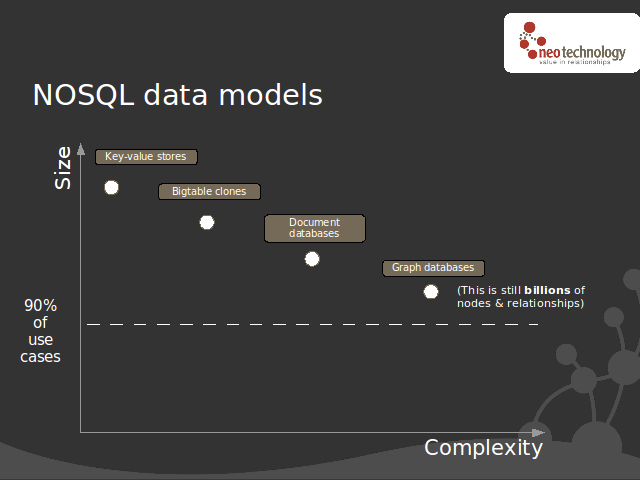
\includegraphics[width=16cm]{./figures/nosqldatamodels.png}
 % topologies802154.png: 722x407 pixel, 72dpi, 25.47x14.36 cm, bb=0 0 722 407
 \caption{Pozícia dátového modelu z pohľadu jeho škálovania podľa veľkosti a komplexnosti. Zdroj: Neo4J a NOSQL overview and the benefits of graph databases, Emil Eifrem, prezentacia.}
 \label{fig:scalling}
\end{figure}

Dátový model typu kľuč-hodnota a stĺpcovo orientovaný model (Bigtable clones) majú jednoduchú štruktúru, ktorá sa dá horizontálne škálovať. Nevýhodou tohoto prístupu je naopak to, že všetká práca s dátami a ich štruktúrou sa prenáša do vyšších vrstiev, o ktoré sa musí starať programátor. Naopak dokumentový a grafový model poskytuje bohatšiu štruktúru na prácu s dátami, ktorá spôsobuje komplikovanejšie škálovanie vhľadom na veľkosť dát. Podľa odhadov spoločnosti Neotechnology až 90\% aplikáci, v prípade že sa nejedná o projekty spoločností Google, Amazon atď., spadá do rozmedia kde sa veľkosť záznamov pohybuje rádovo v miliardách. Za zmienku stojí fakt, že aj napriek tomu, že tieto dátové modely sú si navzájom izomorfné, vhodnosť ich použitia závisí na konkrétnom príklade a požiadavkoch na aplikáciu. 

%one size fits all?
\subsection{Elastickosť}
Vďaka horizontálnemu škálovaniu sa snažime o zýšenie kapacity celkového dátového úložiska. Elastickosť škálovania popisuje ako sa daný systém dokáže vysporiadať s pridaním alebo odobraním uzlu. U tejto vlastnosti sledujeme či je potrebné manuálne rebalancovanie dát, reštartovanie celého systému alebo zmena v uživateľskej aplikácii. Táto vlastnosť by ideálne mala zabezpečiť lineárne zvyšovanie výkonu u operácií ako je čítanie alebo zapisovanie dát.


\subsection{Konzistencia dát}
Poďla teórie CAP platí, že v prípade výskytu sieťových prerušení, ktoré sú súčasťou distribuovaného databázového systému nie je možné súčasne zaručiť vlasnosť konzistencie a dostupnosti. NoSQL systémy preto môžeme rozdeliť podľa tohoto modelu.

\begin{figure}[h]
 \centering
 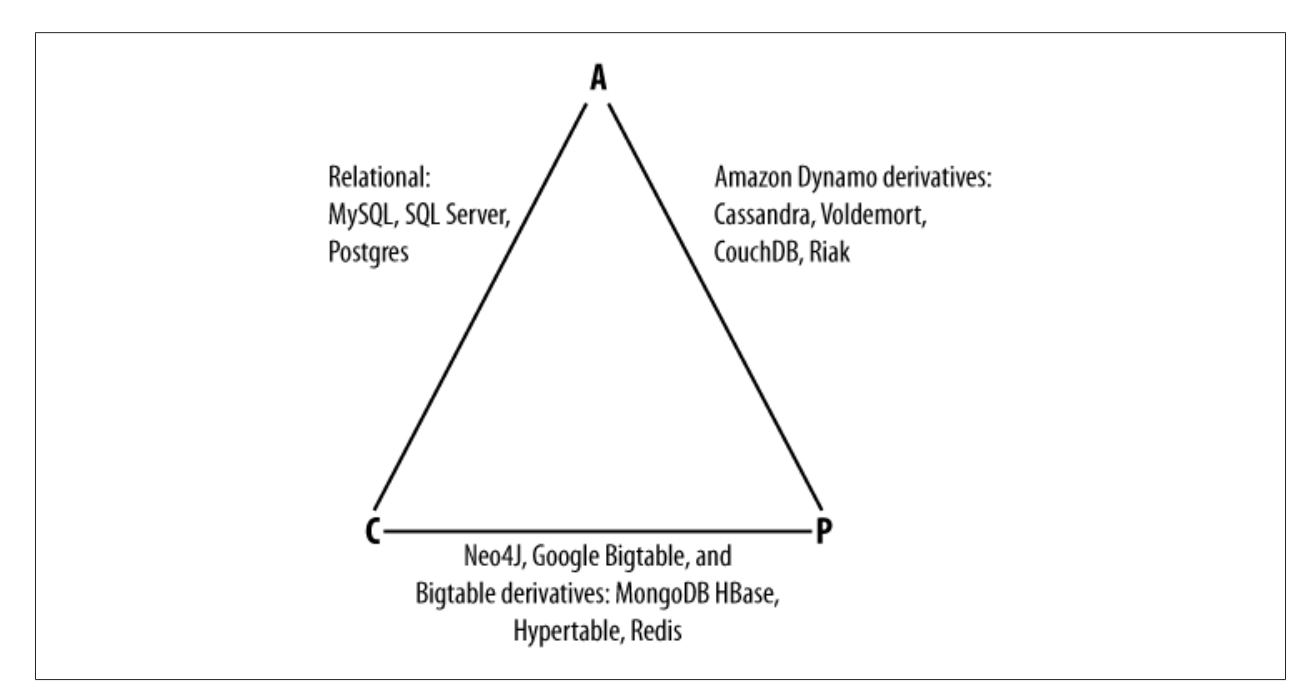
\includegraphics[width=16cm]{./figures/capDatabases.png}
 % topologies802154.png: 722x407 pixel, 72dpi, 25.47x14.36 cm, bb=0 0 722 407
 \caption{}
 \label{fig:scalling}
\end{figure}

Umiestnenie niektorých NoSQL datázových systémvo sa môže meniť podľa ich konfigurácie. 

Podpora replikácie, rozsekávania dát a zaradenie systému podľa modelu CAP určuje jeho dostupnosť.

\subsection{Perzistentné úložisko}
Typ perzistentného úložiska popisuje interný spôsob ukládania dát v databázovom systéme. NoSQL systémy môžu používať na ukládanie dát následujúce štruktúry: 
\begin{itemize}
 \item B-stromy
 \item distribuované hešové tabuľky
 \item Memtable / SSTable \footnote{Tieto štruktúry popíšeme v následujúcej sekcii}
 \item spojové zoznamy
 \item operačná pämeť, ktorej obsah je pravidelných intervaloch ukládaný na pevný disk
\end{itemize}
 
Podľa požiadavkov na našu aplikáciu sme čiastočne schopný odhadnúť pomocou, ktorej štruktúry by sme mohli dosiahnúť čo najefektívnejšiu výkonnosť.


%Snaha o globlálne výkonostné testy NoSQL systémov by viedla k porovnávaniu \uv{jabĺk s hruškami}.
%V následujúcej sekcii využijeme Yahoo! Cloud Serving Benchmark pre porovnanie nami vybraných kandidátov.

\section{Výber NoSQL systémov}
%http://themindstorms.blogspot.com/2009/05/quick-reference-to-alternative-data.html
%http://www.metabrew.com/article/anti-rdbms-a-list-of-distributed-key-value-stores

V predchádzajúcej sekcii sme tieto systémy rozdelili do štyroch hlavných kategórií podľa ich dátového modelu, ktorý je kľúčový pri výbere vhodného databázového systému podľa požiadavkov aplikácie. Popis a výkonnostné porovnanie NoSQL systémov, ktoré reprezentujú jednotlivé kategórie by boli nad rámec tejto práce. Paralelne s touto prácou vzniká diplomová práca, ktorá rieši podobný problém s využitím dokumentových databázových systémov  \ref{barina}, preto túto kategóriu vynecháme.

NoSQL systémy môžeme rozdeliť podľa toho v akom prostredí pracujú. Väčšina týchto systémov vyžaduje ich inštaláciu na počítačové systémy, patria sem napríklad Voldemort, Cassandra, Riak, Hbase. Tieto systémy sú open-source. Okrem nich existujú distribuované databázové systémy, ktoré sú poskytované ako cloudové riešenie a to Amazon SimpleDB,  Microsoft Azure SQL, Yahoo! YQL a prostredie od spoločnosti Google AppEngine. Tieto systémy poskytujú priamo rozhranie na prácu s dátami a funkčnosť perzistentného úložiska zabezpečujú poskytovatelia týchto služieb. Ich hlavným cieľom je zefektívnenie vývoja a nasadzovania aplikácií.

Podľa analýzy požiadavkov na našu aplikáciu a štruktúry dát, ktoré budeme do databázového systému ukládať nie je vhodné použitie databázových systémov s grafovým modelom a modelom kľúč-hodnota. Systémy s grafovým modelom sú určené na diametrálne odlišnú úlohu problémov naopak v prípade, použita systémov kľúč-hodnota by bola práca na strane aplikácie zbytočne náročna. Našim požiadavkom najlepšie vyhovuje stĺpcovo orientovaný model, ktorý sme sa rozhodli použiť pre návrh našej aplikácie.

V tejto časti práce sa zameriame na stručný prehľad a vzájomné porovnanie systémov, ktoré poskytujú stĺpcovo orientovaný model. Medzi tieto voľne dostupné (open-source) systémy patria HBase, Cassandra a Hypertable. Aj napriek totožnému dátovemu modelu, majú tieto systémy odlišné vlasnosti. Následujúca tabuľka zobrazuje popis vlasností, na ktoré sme sa zamerali pri výbere víťaznej dvojice.

\begin{table}
    \begin{tabular}{|l|l|l|l|}
        \hline
        Vlastnosti/Databázový systém & Hbase & Cassandra & Hypertable \\  \hline
        Distribuovaný systém	& áno  & áno & áno \\ \hline 
        Dátový model		& Bigtable \footnote{lala} & Bigtable & Bigtable \\ \hline
        Dotazovací model	& ~  & ~ &  \\ \hline
	Klient 			& Thrift, REST  & Thrift, Avro & Thrift, C++ \\ \hline
        Perzistentné úložisko	& HDFS  & LSS\footnote{lokálny súborový systém} & HDFS, KFS, LSS \\ \hline
        SPOF \footnote{SPOF - uzol, ktorého nedostupnosť spôsobí nedostupnosť celého systému}	& áno  & nie & áno \\ \hline
	Pridanie uzlu do živého systému & áno  & áno & ~ \\ \hline
	Podpora viacerých datacentier & áno  & áno & áno \\ \hline
	Rozsekávanie dát 	& áno  & áno & áno \\ \hline
        Replikácia 		& pomocou HDFS  & áno & áno \\ \hline
	Elastickosť	        & áno  & áno & ~ \\ \hline
	Konzistencia 		& CP  & AP & ~ \\ \hline
	Programovací jazyk 	& Java  & Java & C++ \\ \hline
	MapReduce 		& áno  & áno & áno \\ \hline
	Komunita 		& +  & +  & - \\ \hline
    \end{tabular}
\end{table}


%porovnavane systemy sme vybrali podla citu , a taktiez spravyme benchmark od yahoo na 2 vybrane

Z porovania je vidieť, že systémy obsahuju množstvo spoločných vlastností. Pri výbere systémov sme zohľadnili aj ich praktické využitie spoločnostiami pôsobiacimi na trhu v produkčných podmienkách. Systém Cassandra je používaný spoločnosťou Facebook v aplikácii na súkromnú poštu. Medzi ďalšie požiadavky patrili podpora komunity, dokumentácia a vývojový cyklus týchto systémov. Z týchto systémov sme následne vybrali dva a to HBase a Cassandru. Dôvodom prečo sme zavrhli systém Hypertable je nepostačujúca dokumentácia, málo aktívna komunita a pomalý vývojový cyklus. V následujúcej sekcii popíšeme ich detaily.


\chapter{Cassandra}
%TODO: zadefinovat spotrebny pocitac
%TODO: podla clanku google zadefinovat ze poruchovost HW je taka a taka

Distribuovaný databázový systém Cassandra bol vytvorený pre interné účely spoločnosti Facebook v roku 2007. Cassandra slúžila na vyhľadávanie v súkromnej pošte, poskytovala úložisko pre indexy. Hlavnými požiadavkami na tento systém bolo zvládať miliardu zápisov denne, schopnosť škálovania podľa narástajúceho počtu použivateľov, beh na spotrebných počítačoch a podpora replikácie medzi geograficky oddelenými dátovými centrami. Ďalším požiadavkom bola vysoká dostupnosť, teda aby chyba žiadného uzlu nespôsobila celkovú nedostupnosť systému. Cassandra je teda decentralizovaný systém, kde každý uzol vykonáva tie isté operácie. V roku 2008 bola zverejnená ako open source projekt a je neustále vyvíjaná mnohými spoločnosťami a vývojármi. Tento systém využíva architektonické princípy distribuovaného databázového systému Dynamo od spoločnosti Amazon a zároveň ich kombinuje s dátovým modelom distribuovaného databázového systému Bigtable vytvoreného spoločnosťou Google. V následujúcom texte popíšeme hlavne princípy, na ktorých je tento systém založený.


\section{Dátový model}
Cassandra k dátovému modelu systému Bigtable pridala štruktúru pod názvom \uv{super stĺpec} (angl. super column). Základnou jednotkou dátového modelu je stĺpec. Stĺpec je tvorený názvom, hodnotou a časovým odtlačkom, ktorý využíva Cassandra pri riešení konfliktov. Skupina stĺpcov je identifikovná pomocou unikátneho kľúča a predstavuje riadok, avšak počet a názvy stĺpcov nie je potrebné vopred definovať. Zoradené riadky podľa hodnoty kľučov a v nich zoradené stĺpce obaľuje štruktúra pod názvom \uv{rodina stĺpcov} (ang. column family). Kľúče sú interne reprezentované ako reťazec znakov a zároveň zotriedené. Názvy stĺpcov možu byť viacerých typov ako napríklad Ascii, Utf-8, Byte podľa, ktorých sú zotriedené. Je možné implementovať vlastnú metódu pre triedenie. Riadky obsiahnuté v jednej rodine stĺpcov sú na pevnom disku fyzicky umiestnené v jednom súbore typu SSTable. Je vhodné do rodiny stĺpcov ukládať relevantné záznamy, ku ktorým budeme pristupovať spoločne, čim sa vyhneme zbytočným diskovým operáciam. Operácie nad stĺpcami, ktoré identifikuje daný kľúč sú atomické v rámci repliky. Operácie nad daným riadkom nevyužívajú zamykanie. Voliteľným príznakom, ktorý môžeme u stĺpcu nastaviť je parameter TTL (angl. time to live), ktorý po uplynutí časového intervalu označí dáta za zmazané.

Štruktúra super stĺpec je špecialny typ stĺpca, ktorý je tvorenými obyčajnými stĺpcami. Stĺpec typu super má názov a jeho hodnota je tvorená zoznamom názvov obyčajných stĺpcov. Tento prístup pridáva ďalšiu úroveň v štruktúre. Super stĺpce obaľuje podobná štruktúra pod názvom super-rodina stĺpcov (angl. super column family). 

Keyspace definuje faktor replikácie a jej metódu, ktorá môže byť závyslá poprípade nezávislá na sieťovej topológii. Na keyspace sa môžeme pozerať ako na databázu v relačných databázových systémov obsahujúcu rodiny stĺpcov, ktoré môžeme prirovnať k tabuľkám v relačných databázach.

Aktuálna verzia Cassandri definuje maximálnu veľkosť dát 2GB, ktoré je možné uložit do jedného stĺpca a stanovuje limit dve miliardy pre maximálny počet stĺpcov v jednom riadku. 

%TODO: obrazok


\section{Rozdeľovanie dát}
%vuh1093.pdf
Kľúčovým požiadavkom systému Cassandra je jeho schopnosť škálovania do šírky, čo vyžaduje pridávanie nových uzlov. Tento požiadavok vyžaduje mechanizmus, ktorý zabezpečí dynamické rozdeľovanie dát medzi uzlami systému. Uvažujme príklad, kde máme k dispozícii jeden server obsahujúci veľké množstvo objektov, ku ktorým pristupujú klienti. Medzi server a klientov vložíme vrstvu kešovacích systémov, kde každý z týchto systémov bude zodpovedný pre rýchly prístup k danej časti objektov nachádzajúcich sa na serveroch. Klient teda musí byť schopný určiť, ku ktorém kešovaciemu systému musí pristúpiť v prípade, že chce daný objekt. Predpokladajme, že klientom zabezpečíme výber jednotlivých kešovacím systémom pomocou hešovania s využitím lineárnej hešovacej funkciek (x -> ax + b (mod p), kde p je počet kešovacích systémov). Pridanie nového kešovacieho systému alebo jeho zlyhanie bude mať katastrofálny dopad na funkčnosť systému. V prípade, že sa zmení parameter p, teda počet kešovacích systémov každá položka bude odpovedať novej a zároveň chybnej lokácii. Tento problém rieši elegantne technika pod názvom úplné hašovanie (angl. consistent hashing) \cite{Karger:1997:CHR:258533.258660}, ktorá sa využíva v distribuovaných systémoch pre prácu s distribuovanými hašovacími tabuľkami. Túto techniku taktiež využíva systém Cassandra.

Výstup hašovacej funkcie MD5 reprezentujeme pomocou \uv{kruhu}, kde v smere hodinových ručičiek postupujeme od minimálnej hodnoty hešovacej funkcie (tj. 0) k maximálnej. Každý uzlol v systéme má pridelenú náhodnu hodnotu z tohoto rozsahu, ktorá určí jeho jednoznačnú pozíciu. Identifikácia uzlu v systéme, na ktorý sa uložia dáta reprezentované hodnotou kľúča sa vykoná aplikáciou hešovacej funkcie na dáta reprezentujúce kľúč. Na základe tejto hodnoty je jednoznačne určená pozícia v kruhu a v smere hodinových ručiek je vyhľadaný najbližší uzol. Výhodou tejto metódy je, že každý uzol je zodpovedný za hodnotu kľúčov, ktorých poloha sa nachádza medzi ním a jeho predchodcom. V prípade pridania nového uzlu alebo jeho odobratia, sa zmena mapovania kľúčov v kruhu prejaví len u jeho susedov. Táto technika zároveň prináša nevýhody, medzi ktoré patrí rovnomerná distribúcia dát a vyváženie záťaže. Dynamo tento problém rieši spôsobom kde každý uzol je zodpovedný za viacero pozícií na kruhu, takzvané virtuálne pozície. Cassandra využíva vlastné mechanizmi na monitorovanie záťaže a automaticky presúva pozície uzlov. Taktiež je možné explicitne u každého uzlu stanoviť jeho polohu v kruhu pomocou zadania jeho identifikátora. Tento spôsob je vhodný v prípade, ak vieme predom určiť koľko uzlov bude obsahovať náš systém. V prípade zvyšovania počtu uzlov je možné tieto identifikátory a teda ich polohu v kruhu zmeniť za chodu systému, čím sme schopný opäť dosiahnúť jeho rovnomerné vyváženie. Identifikátor polohy uzlov vieme určiť pomocou následujúceho programu, kde K je počet uzlov v systéme.

\begin{verbatim}
RING_SIZE = 2**127
def tokens(n):
  rv = []
  for x in xrange(n):
    rv.append(RING_SIZE / n * x)
  return rv

print tokens(K)
\end{verbatim}


%TODO Obrazok kruhu


\section{Replikácia}

S úplným hašovaním úzko súvisý replikácia, ktorá zabezpečuje vysokú dostupnosť a odolnosť dát proti ich stráte (angl. durability). Každá dátová jednotka vložená do systému je replikovaná na N uzlov, kde počet N je voliteľne nastaviteľný pre daný keyspace. Každý uzol sa v prípade replikácie N > 1 stáva koordinátorom, ktorý je zodpovedný za replikáciu dát, ktorých kľúč spadá do jeho rozsahu na kruhu. V prípade zápisu koordinátor replikuje dáta na ďalších N - 1 uzlov. Cassandra podporuje viacero spôsobov pre umiestňovanie replík.

\subsection*{Jednoduchá stratégia}

Táto stratégia umiestňuje replikú dát bez ohľadu na umiestnenie serverov v datacentre. Replika dát uzlu je uložená na jeho N-1 susedov v smere hodinových ručičiek. Z toho vyplýva, že každý uzol je zodpovendný za dáta, ktorých kľúče spadajú do jeho rozsahu a taktiež dáta, ktorých kľúče spravuje jeho N predchodcov.

\subsection*{Sieťová stratégia}

Pri tejto metóde a úrovni replikácie s hodnotou aspoň tri, sme schopný zabezpečiť umiestnenie dvoch replík v rozdielnych rackoch, tretia replika bude umiestnená do iného datacentra. Táto stratégia je výhodna v prípade ak chceme použiť časť serverov na výpočty pomocou Mapreduce a zvyšné dve repliky budú slúžiť na obsluhu reálnej prevádzky.

\section{Členstvo uzlov v systéme}

Distribuovaný systém musí byť schopný odolávať chybám ako porucha uzlov alebo sieťové prerušenia. Podpora decentralizácie a detekcia chýb využíva mechanizmi založené na gosship protokoloch. Tieto protokoly slúžia pre vzájomnú komunikáciu uzlov vymnieňajúcich si navzájom doležité informácie o svojom stave. Periodicky v sekundových intervaloch každý uzol kontaktuje náhodne vybraný uzol, kde si overí či je tento uzol dostupný. Detekcia možného zlyhanai uzlu je realizovaná algoritmom s názvom Accrual Failure Detector \cite{accrualdetector}.

Pridávanie novýchu uzlov, presun uzlov v rámci kruhu a iné operácie sa taktiež dejú pomocou Gosship protokolu. Tento protokol zabezpečuje, že každý uzol obsahuje informácie o tom, ktorý uzol je zodpovedný za daný rozsah kľúčov v kruhu. Ak sa vykonáva operácia čítania alebo zápisu dát na uzol, ktorý nie je zodpovedný za tento kľúč, dáta sú automaticky preposlané na správny uzol s časovou zložitosťou O(1).

\section{Perzistentné úložisko}

Tento systém bol primárne navrhnutý tak aby spracúval vysoký tok dát pre zápis, s tým že čo najmenej ovlplyvní efektívnosť operácií na čítanie. Cassandra využíva ako perzistentné úložisko dát lokálny súborový systém. 

\section{Konzistencia}

Konzistencia systému je maximálne konfigurovateľná a využíva princípy techník založených na protokoch kôra. Klient si môže nastaviť hodnotu R určujúcu koľko replík musí potvrdiť úspešnosť operácie čítania dát. Hodnota W určuje na koľko replík je potrebné vykonať zápis a následne vrátiť potvrdenie o jeho úspešnosti klientovi. V prípade, že platí vzťah R + W > N, kde N je počet replík tak sa jedná o silne konzistentný systém, naopak v prípade voľby klienta, kde R + W < N, sa jedná o slabú konzistenciu čím zaručíme vysokú dostupnosť.

\section{Zápis dát}
Ak uzol obrží požiadaok pre zápis, dáta sú zapísané do štruktúry pod názvom commit log, ktorá je uložená na lokálnom súborovom systéme a zabezpečí trvácnosť dát. Zápis do tejto štruktúry je vykonávaný sekvenčne čo umožnuje dosiahnúť vysokú priepusnosť. Dáta sú následne nahrané do štruktúry pod názvom memtable, ktorá sa nachádza v operačnej pamati a v prípade, že by tento zápis zlyhal alebo by došlo k neočakávanému zlyhaniu inštancie Cassandri je možné ich obnovenie z commit logu. Po dosiahnutí určitéh prahu, tj. počtu dát uložených v memtable sú tieto štruktúry asynchrónne zapísané do štruktúr pod názvom SSTable (Sorted String Tables), ktoré už nie je možné modifikovať pomocou aplikácie. Štruktúry SSTables sa následne zlievajú v pravidelných intervaloch na pozadí počas behu, táto operácia je neblokujúca. Počas zlievania SSTables dochádza k zotriedenému zlievaniu kľúčov, k nim prinaležiacím dát, odtraňovaniu dát určených na vymazanie a generovaniu nových indexov. Taktiež dochádza ku generovaniu štruktúr pod názvom Bloom filters\footnote{http://en.wikipedia.org/wiki/Bloom\_filter} pre každú SSTable.

Zápis dát nevykonáva žiadne diskové operácie, ktoré by potrebovali čítať dáta, je atomický pre danú ColumnFamily a v prípade, že systém Cassandra beží je stále dostupný a rýchly.

%sstable data,index,filter?
%http://wiki.apache.org/cassandra/ArchitectureOverview

\section{Čítanie dát}
V prípade požiadavku na načitanie dát, sa požadované dáta najprv hľadajú v štruktúrach memtable, ktoré sú uložené v operačnej pamati. Ak sa dané data nenachádzajú v operačnej pamati, vyhľadávanie sa uskutočnuje podľa kľúča v diskových štruktúrach SSTable. Kedže snahou systému je čo najefektívnejšie vyhľadávanie, využívajú sa bloom filtre. Bloom filtre sú nedeterministické algoritmy, ktoré dokážu otestovať či element patrí do množiny. Napriek ich nedeterminizmu generujú len falošné pozitíva. Pomocou nich je možné namapovať kľúče zo štruktúr SSTables do bitových polí, ktoré je možné uchovať v operačnej pamati. Vďaka tomu sa redukuje prístup na disk, keď hľadáme súbor, ktorý obsahuje dáta odpovedajúce hľadanému kľúču. Požiadavok pre čítanie dát možeme zaslať na ľubovoľný uzol.

\section{Zmazanie dát}
Keď vykonáme operáciu reprezentujúcu zmazanie dát, tieto dáta sa nevymažú okamžite. Namiesto toho sa vykoná operácia, ktorá dané dáta označkuje príznakom pod názvom tombstone. Po uplynutí doby, ktorá je štandardne nastavená na desať dní, sa tieto dáta odstránia pri procese zlievajúcom štruktúry SSTables.


\section{Bezpečnosť}

Implicitne Cassandra nevyužíva žiadne prvky, ktoré by poskytovali možnosť znemožnenia prístupu k dátam v nej uložených. K dispozícii je modul, ktorý umožnuje nastavenie auntentizácie na úrovni Keyspace-u pomocou textových hesiel alebo ich MD5 odtlačkov. Obmedzovanie prístupu k datám je preto potrebné zabezpečiť na aplikačnej úrovni.




%%%%%


%obmedzenie MYSQL = +papier 5
%mysqlscalling and high avail.pdf -

% 
% Musime predpokladat ze zlyhania v tak velkej infrastrukture su bezna vec a nie ojedinela zalezitost = HW a siet zlyhania
% Zapis nie je nikdy rejectnuty(ani v pripade hw poruchy ani v pripade concurent writes),  z tho odovodu je to alway writtable system = co ale implikuje ze konflikty sa riesia pocas operacie READ
%   riesenie konfliktu na strane db vyuziva jednoduche techniky = last write win, kdezto na strane klienta napriklad mozeme pouzit merge na 2 rozne verzie dat (nakupny kosik)
% bigtable = multi dimensional sorted map
% Zero hop DHS = kazdy uzol obsahuje dostatok informacii na priame presmerovanie poziadavku na cielovy uzol 
% 
% kluc je array of bytes na neho sa aplikuje mdť hash ktory vygeneruje +ľábit identifikator na zaklade ktore sa urci uzol kde budu ulozene data pre dany kluc
% 
% partitioning = consistent hashing = najvacsia hodnota has funkcie v spojeni s najnizsou (0) vytvori kruh na ktory sa umiestnia jednotlive uzly.... data sa potom podla md5(key) umiestnia na dany uzol (v smere hod ruciciek ktoreho  pozicia ja vacsia ako pozicia md5(kluca) Kazdy uzol je takto zodpovedny za svoj region (uzol => predchodca) ... vyhodou konzistent hashovania je ze havaria/pridanie noveho uzla ovplyvňuje len susedov. Tento koncept obsahuje viacero nedostatkov ako napriklad nerovnomerna distribucia zataze.... 
% preto sa aplikuje upraveny consistent hasing a to tak ze kazdy uzol obsahuje viacero virtualnych pozicii na ringu
% 
% 
% Replikacia zabezpecuje hlavne dostupnost a stalost dat {durability}
% 
% 214: W a R impact object availability durability and consistency 
% N R W - 3,2,2 podla dynamo paper {215}
% 
% distirbucia klucov pri malej zatazi - horsie to loadbaloncovalo ako pri velkej zatazi  215
% 209 tabulka + obrazok
% 
% diskusia nad n,r,w 214
% 
% 
% 
% 
% detekcia konfliktov pri upgrade pomocou vector clock - ale kedze mi len WRITE nezaujima nas to
% v pripade ze preda dany stlpec nemame hodnotu nic sa nikam nezapisuje
% 
% 
% kapitola impl -- v pripade ze nejaka polozka neexistuje nic sa nedeje ... neukladame ... handlujeme na strane klienta
% %Rodina stlpcov - last 100 emails , je automaticky zotriedena podla datumu, co podporuje samotna Cassandra.
% Hardware failure is the norm rather than the exception.

\chapter{HBase}
% podla porovnania vybereme 2 a tie dosledne popiseme 
% dovod preco sme vybrali column.familly - graf = komplexnost problemu narast data = a podla neho ze nepotrebujem key-value - zlozita praca so strukt. datami...  a popis 2 vybranych
V tejto kapitole stručne popíšeme distribuovaný súborový systém, ktorý je súčasťou projektu Hadoop a zároveň slúži ako perzistentné úložisko pre distribuovanú databázu HBase. Následne popíšeme základné princípy fungovania tohoto databázového systému.

\section*{Hadoop}
%shvachko.pdf

Hadoop\footnote{http://hadoop.apache.org/} je open source projekt v programovacom jazyku Java, ktorý tvorý distribuovaný súborový systém HDFS (Hadoop Distributed Filesystem) a framework MapReduce pre spracúvanie objemu dát v desiatkách PB \cite{Thusoo:2010:DWA:1807167.1807278}. Medzi hlavné požiadavky tohoto systému patria vysoká dostupnosť, škálovateľnosť a distribuovaný výpočet. Architektúra HDFS vychádza z princípov distribuovaného súborového systému Google File System\cite{Ghemawat:2003:GFS:945445.945450} (GFS) a pôvod frameworku MapReduce pochádza taktiež od spoločnosti Google\cite{Dean:2008:MSD:1327452.1327492}.

 
%kto ho pouziva a na ake typy appl


Súborový systém využíva architektúru master-slave. Uzol master, pod názvom Namenode, udržiava v operačnej pamäti metadata, ktoré popisujú štruktúru súborov, adresárov, reprezentujú mapovanie súborov na bloky a určujú ich umiestnenie na uzloch Datanode. HDFS predpokláda prácu so súbormi rádovo v desiatkách gigabajtov, ktoré sú interne reprezentované dátovými blokmi o štandardnej veľkosti 65 MB. Tieto bloky sú uložené v uzloch typu slave, ktoré sa nazývajú Datanode. Klient v prípade načítania súboru kontaktuje Namenode, ktorý mu poskytne informácie, na ktorých uzloch typu Datanode sa nachádzajú bloky reprezentujúce súbor a dátová komunikácia následne prebehne medzi klientom a uzlom Datanode. HDFS je optimalizovaný pre jednorázový zápis dát a ich následné mnohonásobné čítanie. Bloky sa replikujú na uzly Datanode. Štandardne je nastavená úroveň replikácie na hodnotu tri, teda každý blok je uložený trikrát.

%TODO popisat format metadat ???

Hlavným nedostatkom tejto infraštruktúry je fakt, že uzlol Namenode tvorí kritický bod systému, v prípade jeho nedostupnosti nie je možné pracovať s HDFS a prípadná strata dát na tomto uzle spôsobí totálne zlyhanie súborového systému bez možnosti jeho obnovy. Súborový systém nie je vhodný pre ukladanie veľkého počtu malých súborov.
Uzol Namenode alokuje pre objekt typu blok a objekt typu súbor 300 B metadát. V prípade uloženia súboru, ktorý nepresahuje veľkosť jedného bloku je potrebné alokovať 300B dát. Ak uložíme 10,000,000 takýchto súborov veľkosť metadát, ktoré udržiava Namenode v operačnej pamati zaberie 3 GB. Celkový počet uložených súborov je obmedzený veľkosťou operačnej pamati RAM, ktorou disponuje uzol Namenode.

Z týchto pozorovaní vyplýva fakt, že distribuovaný súborový systém HDFS nemá praktické využitie ako úložisko dát slúžiace k archivácii emailových správ, pre ktoré sme zadefinovali požiadavky v tretej kapitole. %TODO:REF
% 
% SYNC!!! a zapis pipeline style  page 69 hadoop book
% 
% Decisions related to the replication of blocks are always taken
% by NameNode, which receives regularly from each DataNode
% in the cluster Heartbeat information and the proportion
% between the blocks used. The information about a file has the
% form [5]:

%NameNode (File_name,Id_blocs, ...)
%replica_numbers, For exemple the next information:
%/path/part-0,r:2,{1,3},...
%/path/part-0,r:3,{2,6,34},..
% means that part-0 is stored with 2 replicas on the blocks 1 and 3, and 3 replicas on the blocks 2, 6, and 34. The strategies
% for replicas place are more important for performance and aviability of HDFS. The usual replication policy is to have two replica machines from the same rack and a replica for a node located in another rack. This policy limits the writing traffic between racks and the chance of failure of the entire rack is much lower than the chance of failure of a node


\section*{HBase}

%replikovanie in pipeline

%TODO REf na bigtable?
Aplikácie ako HDFS alebo MapReduce slúžia na dávkové spracúvanie obrovského objemu dát. HBase je open source, distribuovaný, stĺpcovo orientovaný databázový systém, ktorý umožnuje prístup k veľkému objemu dát a ich zápis v reálnom čase. Ako perzistentné úložisko dát využíva distribuovaný súborový systém HDFS, je taktiež implementovaný v Jave a jeho architektornické koncepty vychádzajú z článku Bigtable od spoločnosti Google. HBase bol vytvorený spoločnosťou Powerset na konci roka 2006, pre potreby spracúvania obrovského objemu dát\cite{White:2009:HDG:1717298} a začiatkom roka 2008 sa stal oficiálnym podprojektom systému Hadoop.

\section{Dátový model}

Dátový model je totožný s konceptom Bigtable. Dáta s ktorými pracuje HBase sa ukladajú do tabuliek. Každá tabuľka obsahuje riadky identifikované kľúčom, ktoré môžu byť tvorené ľubovoľným počtom stĺpcov. Klúče sú reprezentované ako pole bajtov (Java byte[]), preto je možné použiť ľubovoľný typ dát napríklad reťazec alebo serializovanú dátovú štruktúru (JSON). Riadky sú radené podľa názvov kľúčov. Stĺpce sú organizované do skupín, ktoré sa nazývajú \uv{rodiny stĺpcov} (angl. column families). Obsahu každej bunky, ktorej pozíciu určuje riadok a stĺpec prináleži verzia, ktorá je reprezentovaná časovou značkou a jej obsah je reprezentovaný ako pole bajtov. Časovú značku určuje klient pri zápise dát alebo je automaticky generovaná systémom HBase (zýskava ju z operačného systému??) Obsah buniek tabuľky je možné sprístupniť pomocou kľúča a názvu stĺpca alebo pomocou kľúča, názvu stĺpca a časovej značky. V prípade uloženia viacerých verzií v danej bunke, sú tieto dáta radené od najaktuálnejšej časovej značky po najstaršiu. 
%ref na hbase architecture pages

Dôležitým faktom je, že stĺpce, ktoré patria do rovnakej rodiny stĺpcov sú fyzicky uložené na tom istom mieste. Rodiny stĺpcov je potrebné zadefinovať počas vytvárania tabuliek. Ich názvy a počet je potrebné vhodne premyslieť už pri samotnom návrhu databázovej schémy. V prípade, že klaster HBase obsahuje viacero uzlov je na nich potrebné zabezpečiť sychronyzáciu systémového času. V prípade veľkého časového rozdielu hrozí, že daná inštancia systému HBase sa nespustí.

%TODO obrazok
%pridavanie CF za behu u C 

\section{Architektúra systému}

HBase využíva architektúru master-slave. Uzol v role master sa nazýva HBase Master, uzly slave RegionServers. Pre chod systému je ďalej potrebná služba Zookeeper {ref + pre synch?}. 

%Zookeeper vyber-urcenie mastra

\subsection*{HBase master}

Tento uzol v systéme vykonáva priradzovanie regiónov RegionServer-om, detekujem pridanie nového RS, jeho zlyhanie a balancuje záťaž na RS v prípade rozdelenia regiónu.

\subsection*{RegionServer}

Region server sĺúži pre obsluhu klientských požiadavkov, samotný zápis alebo čítanie dát sa vykonáva medzi klientom a RS. Každý RS spravuje niekoľko regiónov, automaticky rozdeľuje regióny a informuje o tom uzol HBase master. Tieto uzly môžeme v systéme ľubovoľne pridávať alebo odoberať počas jeho prevádzky.

%TODO> testovanie aktualne su clanky zle popisy konfiguracii chybaju udaje o RF atd..
%zle metodologie 

\section{Rozdeľovanie dát}

Základnou jednotkou, ktorá zabezpečuje rozdeľovanie dát a teda umožnuje horizontálne škálovanie a rovnomerné rozloženie záťaže v klastri je region. Region má náhodne vygenerovaný identifikátor a tvorí ho interval riadkov, kde posledný riadok do daného intervalu nepatrí. Tabuľka je tvorená regiónmi, pri jej prvotnom vytvorení ju zvyčajne reprezentuje jeden región. V prípade, že jej veľkosť dosiahne predom stanovenú hranicu (závyslé na konfigurácii), dojde k rozdeleniu riadkov do dvoch nových regiónov s podobnou veľkosťou. Tieto regióny sú  v klastri distribuované na uzly typu RegionServer. Tento mechanizmus zabezpečuje, že do systému je možné uložiť tabuľku, ktorej veľkosť by nebolo možné spracovať pomocou jedného fyzického počítača.

Región je základný element, ktorý zabezpečuje dostpnosť a rovnomerné rozloženie záťaže.

\section{Replikácia}
%http://hbase.apache.org/replication.html
HBase podporuje replikáciu v rámci viacerých geograficky oddelených datacentier. Replikácia funguje na rovnakom princípe ako v databázovom systméme MySQL \footnote{http://dev.mysql.com/doc/refman/5.1/en/replication-formats.html}, teda master-slave a je asynchrónna. Táto forma replikácie zanáša do daného distribuovaného systému eventual consistency na strane uzlov typu slave.

%priklad pouzitia - real data vs. m/r

Primárnu replikáciu dát, ktorá zabezpečuje silnú konzistenciu a zabraňuje stráte dát je možné zabezpečiť pomocou perzistentného úložiska, v tomto prípade na úrovni HDFS.

%TODO datacentra


\section{Perzistentné úložisko}

Tento distribuovaný databázový systém je schopný pracovať v lokálnom móde, kde vyššie spomínané komponenty bežia ako samostatné služby na jednom fyzickom uzly a ako úložisko sa využíva lokálny súborový systém.

V prípade distribuovaného módu rozlišujeme dva typy:
\begin{itemize}
 \item pseudo distribuovaný mód, kde všetky komponenty bežia na jednom uzly
 \item distribuovaný mód, jednotlivé komponenty bežia na samostatných uzloch
\end{itemize}

Obidve konfigurácie môžu využívať ako perzistentné úložisko distribuovaný súborový systém HDFS, KFS alebo Amazon S3. Štandardne sa doporučuje použitie HDFS.

\section{Konzistencia}

Systém sa vyznačuje silnou konistenciou. Z modelu CAP splňuje CP, teda uprednosňuje konzistenciu pred dostupnosťou.


\section{Zápis dát a čítanie dát}

V prípade zápisu alebo čítania dát klient kontaktuje ZK, od ktorého obrží informáciu o lokácii tabuľky -ROOT- a následne kontaktuje daný RS obsahujúci túto tabuľku. Z tabuľky -ROOT- sa určí RS, ktorý obsahuje tabuľku \uv{.META.}, tieto kroky sa lokálne kešujú na strane klienta. Následne klient kontaktuje daný RS a v tabuľke .META. vyhľadá uzol obsahujúci región, do ktorého patria hľadané alebo zapisované dáta. V poslednom kroku prebieha všetká dátová komunikácia medzi klientom a posledným vyhľadaným uzlom.

S týmto RS následne prebieha dátová komunikácia. Dáta sú zapísané do štruktúry HLog (typu WAL), ktorá je uložená na HDFS. Po potvrdení o úspešnom zápise sú data nahrané do štruktúry MemStore, ktorá je uschovaná v operačnej pamäti. V  prípade, že RegionServer obrdží požiadavok na čítanie dát, dáta sú načítane buď zo štruktúry MemStore alebo HFile.

%TODO obrazok
% 
% Hlog per RS and in HDFS
% HLog is the HBase WAL implementation, and there is one HLog instance per RegionServer.
% 
% http://www.larsgeorge.com/2009/10/hbase-architecture-101-storage.html
% http://th30z.blogspot.com/2011/02/hbase-io-hfile.html?spref=tw
% http://www.larsgeorge.com/2010/05/hbase-file-locality-in-hdfs.html
% Schubert Zhang's blog post on HFile: A Block-Indexed File Format to Store Sorted Key-Value Pairs makes for a thorough introduction to HBase's hfile.
%KESOVANIE --- celej identifikacie Regionou<
Zápis alebo čítanie dát na úrovni riadku identifikovaného pomocou kľúča je atomická operácia. 
\section{Zmazanie dát}

U operácii zmazania dát je potrebné špecifikovať či chceme zmazať dáta staršie určitá časová značka poprípade dáta odpovedajúcej konkrétnej časovej značke. Keď vykonáme operáciu reprezentujúcu zmazanie dát, tieto dáta sa nevymažú okamžite z dôvodu, že štruktúry HFile sú po zápise nemenné a aby sa nevykonávali zbytočné diskové operácie. Namiesto toho sa vykoná operácia, ktorá dané dáta označkuje príznakom pod názvom \uv{tombstone}. Tieto dáta odstránia pri procese zlievajúcom štruktúry HFile.


%TODO:
%Bulkload? http://hbase.apache.org/bulk-loads.html
%TTL<


\section{Bezpečnosť}

Distribuovaný databázový systém je možné nasadiť do claudu. V prípade, použitia verejných audov môže hroziť nebezpečenstvo zneužitia našich dát treťou stranou a preto je potrebné aplikovať bezpečnostné mechanizmi. Pri nasadení systému do privátneho klaudu zasa môžeme požadovať viacero úrovní ochrany pre prístup k dátam. Hadoop a HBase aktuálne poskytujú prvok autentizácie pomocou Kerberosu. Možnosť pridania autorizácie na úrovni tabuliek a rodiny stĺpcov je neustále vo vývoji. 


Secure HBase, Hadoop Group  Trend Micro: Andrew Purtell, Gary Halmling, Joshu Ho, Eugene Koontz, Mingjie Lail
http://www.slideshare.net/ghelmling/secure-hbase-hw2010

https://issues.apache.org/jira/browse/HBASE-1697
https://issues.apache.org/jira/browse/HBASE-3025

http://hbaseblog.com/2010/10/11/secure-hbase-access-controls/
http://hbaseblog.com/2010/07/21/up-and-running-with-secure-hadoop/



% 
% 
% 
% LZO , GZIP
% 
% v uvode sme predpokladali ze na testovanie pouzijeme YCSB .. ale jeho ... badass
% 
% 
% TODO: Describe how YCSB is poor for putting up a decent cluster load.
% 
% TODO: Describe setup of YCSB for HBase


\chapter{Testovanie výkonnosti}

Výkonové porovnanie NoSQL systémov je zložitá úloha, neexistuje univerzálny nástroj, ktorým by bolo možné tieto systémy navzájom porovnať. 
Tieto systémy sa vyznačujú rôznými vlastnosťami ako typ konzistencie, dostupnosť, optimalizácia pre zápis alebo čítanie a ich výber závisí na prípade použitia. Všeobecný nástroj pre ich porovnanie by preto nemal žiadne opodstatnenie. Taktiež nie sú k dispozíci žiadne všeobecné techniky, ktorými by bolo možné testovať napríklad konzistenciu týchto distribuovaných systémov, spoľahlivosť a iné. Výkon týchto systémov môže ovplyvňovať faktor replikácie, spôsob rozdeľovania dát alebo úroveň konzistencie. Veľmi častou a zároveň časovo náročnou metódou, ktorá slúži na porovnávanie týchto systémov je implementácia daného riešenia s využitím všetkých porovnávaných systémov. V tejto kapitole sa zameriam na popis výkonnostných testov, ktoré som vykonal v reálnych podmienkach a pri ktorých som pozoroval ako systémy HBase a Cassandra zvládajú vysoký zápis v rôzných konfiguráciách faktoru replikácie, počtu uzlov v klastri a úrovňou konzistencie.

%TODOpokusime sa najst spojitost_ overit : 

\section{Testovacie prostredie}

Pre výkonnostné testovanie som mal k dispozícii 9 počítačov s rovnakou hardvérovou a softvérovou konfiguráciou, ktoré boli navzájom prepojené pomocou 10 Gbit smerovača a komunikovali po 1 Gbit linke. Konkrétnu softvarovú konfiguráciu testovaných aplikácií popíšem jednotlivo v nasledujúcich podkapitolách.

\subsection*{Hardvérová konfigurácia}
\begin{itemize}
 \item 4 jádrový procesor Intel, 5506@2.13Ghz
 \item 4 GB RAM
 \item 5 pevných diskov (SATA, 7200RPM) o veľkosti 1TB zapojených v poli RAID0
 \item 1 Gbit sieťová karta
\end{itemize}

\subsection*{Softvérová konfigurácia} 
Každý uzol obsahoval inštaláciu operačného systém Debian GNU/Linux Lenny x64, Sun Java JDK 1.6.0\_+88. Na každom uzle bol deaktivovaný odkladací priestor (angl. swap). Za účelom monitorovania bol použitý softvér Zabbix, VisualVM, htop, iostat a dstat.

\subsection*{Sieťová konfigurácia}

Hodnota maximálnej reálnej sieťovej priepustnosti medzi dvoma uzlami bola zmeraná pomocou aplikácie nuttcp\footnote{http://www.wcisd.hpc.mil/nuttcp/} s výslednou hodnotou 940 Mbit.

\section{Popis testovacej metodológie}

Nad oboma distribuovanými databázovými systémami sme vykonali testy na základe, ktorých sme sa snažili identifikovať ako tieto systémy ovplyvňuje rôzna úroveň replikácie, konzistencie, pozorovali sme ich schopnosť horizontálneho škálovania a chovanie sa pod záťažou. Testy boli zamerané na zápis dát, ktorý je kritickým prvkom pre potreby našej aplikácie.

\subsection{Testovací klient}

Testovací klient bol multivláknová aplikácia založená na princípe producent - konzument, kde konzumenti predstavovali jednotlivé vlákna vykonávajúce zápis do databázových systémov. Optimálny počet paralelne zapisujúcich vlákien bol stanovený na hodnotu 50, pri ich zvyšovaní sa zvyšovala latencia a nedošlo k zvýšeniu dátového toku pre zápis. Kritickým bodom bolo v tomto prípade, zabezpečiť počas celej doby jednotlivých testov rovnaké zaťaženie každého uzla v klastri. Detailný popis splňujúci tento bod je obsiahnutý v časti popisujúcej test konkrétneho databázového systému.

\subsection{Testovací prípad pre zápis dát}

V tomto testovacom prípade sme postupne do klastra obsahujúceho jeden, tri a šesť uzlov zapisovali 8,000,000 riadkov. Každý riadok obsahoval jeden stĺpec o veľkosti 1000 B, ktorého obsah tvorili náhodné data. Počet celkovo zapísaných dát bol 7,6 GB. Uzly obsahovali 4 GB fyzickej operačnej pamati a v prípade, zápisu malého množstva dát by tieto dáta nemuseli byť zapísané počas testu na pevný disk, časť ich obsahu by mohla byť uložená v štrukúrach Memtabe a Memstore. Zvolili sme preto cca dvojnásobnú veľkosť zapisovaných dát v porovnaní s veľkosťou operačnej pamati, čím počas testu docielime so 100\% pravedepodobnosťou zaťaženie pevných diskov. Za zmienku stojí fakt, že na Internete sú dostupné články, testujúce tieto systémy, ktoré počas testu neprekročia 1/3 RAM?? \cite{}.

\subsection{Testovací prípad pre čítanie dát}

Dôvodom tohto testovacieho prípadu bolo určiť ako dané systémy zvládajú čítanie dát, pretože pre výpočet štatistík pomocou MapReduce bude mať rýchlosť čítania dát výrazný vplyv na celkovú dobu trvania výpočtov.

\subsection{Zaťažovací test}

Cieľom bolo zistiť stabilitu klastra v prípade, keď bude pod sústavným zápisom, budú v ňom prebiehať časté operácie pre zápis štruktúr Memtable a Memstore na pevný disk a ich následné zlievanie. Tento test sme vykonali po dobu piatich hodín. Počas niektorých testovacích prípadov sme použili dvoch klientov z dôvodu aby sme zaručili maximálnu saturáciu prenosového pásma a vylúčili úzke hrdlo na strane klienta (1 Gbit linka umožňuje maximálny teoretický dátový tok 125 MB/s).




\section{HDFS}
Nad distribuovaným súborovým systémom HDFS sme vykonali testy určujúce maximálnu hodnotu priepustnosti pre zápis dát, z dôvodu aby sme vylúčili možné úzke hrdlo v jeho prepojení s databázovým systémom HBase. Pre účely testovania sme použili verziu Hadoop-0.20.2, veľkosť haldy pre JVM (ang. Java Virtual Machine) bola nastavená na na 1 GB.

Meranie maximálnej rýchlosi zápisu sme testovali v troch konfiguráciach. Každá konfigurácia obsahovala jeden uzol v role master, na ktorom boli spustené služby? Namenode a JobTracker. Na zvyšných uzloch typu slave ?bežali služby Datanode a Tasktracker. Konfigurácia klastrov bola následovná:

\begin{itemize}
 \item A - tri uzly slave s faktorom replikácie jedna
 \item B - tri uzly slave s faktorom replikácie tri
 \item C - šesť uzlov slave s faktorom replikácie tri
\end{itemize}

Počas jednotlivých testov sa na súborový systém zapisovali tri rôzne veľkosti súborov, kde v HDFS bola zachovaná štandardná veľkosť bloku tj. 65MB. 
TODO:rozpisat
Pomocou MapReduce sa na každom uzle typu slave paralelne vykonával zápis súborov o danej veľkosti. Testy boli vykonané nástrojom TestDFSIO a na každý uzol sa zapisovalo 12 GB dát. Každý test bol vykonnaný trikrát a výsledná hodnota bola určená ako aritmetický priemer. Výsledky testu, ktoré zobrazuje tabuľka \ref{tab:HDFSperformance} poukazujú na fakt?, 

\begin{table}[hp]
\begin{center}
\begin{tabular}{|c|c|c|c|}
\hline 
\multirow{2}{*}{Veľkosť súboru [MB]} & \multicolumn{3}{|c|}{Klaster}  \\
\hline & A & B & C\\
\hline 128 & 287 MB/s& 102 MB/s& 190 MB/s\\ 
\hline 812 & 371 MB/s& 85 MB/s& 162 MB/s\\ 
\hline 4096 & 433 MB/s& 85 MB/s& 163 MB/s\\ 
\hline
\end{tabular} 
\end{center}
\caption{Výkonnosť HDFS pre zápis dát}
\label{tab:HDFSperformance}
\end{table}

že zvýšenie faktoru replikácie ma zásadný negatívny vplyv na celkový výkon distribuovaného súborového systému.

Dôležitý fakt, ktorý vyplynul z výsledkov testovania je, že v prípade ak zvýšime dvojnásobne počet uzlov v klastri (prípad klastrovv konfigurácii B a C), jeho výkonnosť vzrastie lineárne, čo potvrdzuje vysokú škálovateľnosť systému. Rôzne veľkosti zapisovaných súborov sme volil s cieľom určiť či daný systém dosahuje lepšie výsledky pre zápis malých alebo veľkých súborov. Počas testov systém nevykazoval žiadne známky preťaženia, nebolo indetifikované žiadne úzke hrdlo.

\section{HBase}
% klaster súbor navzájom prepojených počítačov tvoriacich paralelný počítač
% Superpočítač – Sálový počítač obsahujúci desiatky procesorov, značnú pamäťovú a úložnú
% kapacitu, predurčený na zložité výpočty a simulácie
% link na hbase book


popis toho ze sme pomocou API vytvorili tabulku s tym ze sme ju predrozdelili na viacero prazdnych regionov - kazdy na inom node - load balancing 
HBase currently does not do well with anything about two or three column families so keep the number of column families in your schema low -- nezmyselne testy v paperoch
Compaction is currently triggered by the total number of files under a column family. Its not size based. ako to je v C ? preto vela compactions a write bottleneck?

bloom filtre default nope .. zapli sme 
\begin{table}[hp]
\begin{center}
\begin{tabular}{|c|c|c|c|c|}
\hline Počet uzlov & Replikácia  & Čas & Riadok/sek & Priepustnosť [MB/s]\\ 
\hline
\hline 1 & 1 &  551 & 14519 & 14\\ 
\hline 3 & 1 &  202 & 39613 & 39\\ 
\hline 3 & 3 &  317 & 25110 & 25\\ 
\hline 6 & 3 &  211 & 37864 & 37\\ 
\hline
\end{tabular} 
\end{center}
\caption{Zápis riadkov o veľkosti 1000 B}
\label{tab:HPerf2}
\end{table}



\begin{table}[hp]
\begin{center}
\begin{tabular}{|c|c|c|c|c|c|}

\hline Počet uzlov & Replikácia & Čas & Riadok/sek & Priepustnosť [MB/s]\\ 
\hline
\hline 1 & 1 & 246 & 4069 & 4\\ 
\hline 3 & 1 & 117 & 8561 & 8\\ 
\hline 3 & 3 & 127 & 7936 & 8\\ 
\hline 6 & 3 & 190 & 11904 & 12\\ 
\hline
\end{tabular} 
\end{center}
\caption{Čítanie riadkov o veľkosti 1000 B}
\label{tab:CPerf3}
\end{table}



\begin{table}[htp]
\begin{center}
\begin{tabular}{|c|c|c|c|c|}
\hline
\multicolumn{5}{|c|}{Počet uzlov}  \\
\hline Veľkost riadku & 3 & 4 & 5 & 6\\ 
\hline
\hline 1 KB & 32 & 35 & 36 & \\ 
\hline 10 KB & 31 & 37 & 41 & 49 \\ 
\hline 100 KB & 35 & 43 & 52 & 55\\ 
\hline 512 KB & 25 & 40 & 51 & 63 \\  
\hline 1 MB & 35 & 47 & 53 & 68 \\ 
\hline
\end{tabular} 
\end{center}
\caption{Maximálna priepustnosť klastru v MB/s}
\label{tab:CPerf1}
\end{table}



\section{Cassandra}
% Spoločnosť Yahoo! zverejnila v roku XXX nástroj pod názvom Yahoo!  Cloud Serving Benchmark (YCBS) pre obecné porovnávanie distribuovaných databázových systémov. Tento nástroj je zameraný na meranie výkonu a eleasticity a podporuje rôzne testovacie prípady, ktorými je možné popísať vlastnosti testovanej aplikácie. Medzi tieto prípady patrí napríklad intenzivný zápis, intenzívne čítanie, náhodné vyhľadávanie v databázovom systéme a iné. Keďže sa jedná o maximálne modulárny nástroj, poskytuje zároveň možnosť tvorby vlastných testovacích prípadov. Cieľom tohoto nástroja je obecné porovnanie distribuovaných databázových systémov. 

Distribuovaný databázový systém Cassandra som podrobil viacerým testom, ktorých zámer a výsledky popíšem v následujúcej časti. Testy boli zamerané hlavne na stabilitu systému, sledovali rýchlosť zápisu dát a ako sa táto rýchlosť mení na základe rôzneho počtu uzlov, úrovne konzistencie a replikácie. Pri testovaní bola použitá verzia Cassandra-0-7.3. Adresár obsahujúci súbory typu commitlog bol na samostatnom fyzickom disku, dátový adresár bol na diskoch zapojených v poli RAID0. Veľkosť štruktúry memtable bola 120 MB. Každý uzol zaberal na hašovom kruhu rovnaký úsek.

Tabuľka \ref{tab:CPerf2} obsahuje výsledky z viacerých meraní, pri ktorých sme do systému zapisoval osem miliónov riadkov s jedným stĺpcom o veľkosti 1000 B. Pre zapisované riadky boli použité ako kľúče hodnoty v rozsahu nula až celkový počet riadkov. Počas testovania boli všetky uzly rovnako zaťažené.

\begin{table}[hp]
\begin{center}
\begin{tabular}{|c|c|c|c|c|c|}
\hline Počet uzlov & Replikácia & Konzistencia & Čas & Riadok/sek & Priepustnosť [MB/s]\\ 
\hline
\hline 1 & 1 & One & 338 & 23669 & 23\\ 
\hline 3 & 1 & One & 207 & 38647 & 38\\ 
\hline 3 & 3 & One & 311 & 25723 & 25\\ 
\hline 3 & 3 & Quorum & 351 & 22792 & 22\\ 
\hline 6 & 3 & One & 202 & 39604 & 39\\ 
\hline 6 & 3 & Quorum & 263 & 30418 & 30\\ 
\hline
\end{tabular} 
\end{center}
\caption{Zápis riadkov o veľkosti 1000 B}
\label{tab:CPerf2}
\end{table}

\subsection*{Škálovateľnosť}

Z výsledkov meraní je vidieť, že tento distribuovaný databázový systém je maximálne škálovateľný z pohľadu rýchlosti zápisu. V prípade, keď som zdvojnásobil počet uzlov z troch na šesť (riadok 3,5) vzrástla priepusnosť zápisu o cca 50\%.

\subsection*{Replikácia}

V prípade zvýšenia úrovne replikácie z 1 na 3 sa automaticky znížila rýchlosť zápisu o jednu tretinu.

\subsection*{Konzistencia}

Počas zápisu s konzistenciou kvóra, ktorá zabezpečuje silnú konzistenciu databázového systému, sa rýchlosť znížila podľa očakávaní. V tomto prípade, aby klient obdržal odpoveď o úspešnom zápise museli byt dáta zapísané na dve repliky.

%aky graf pouzit na zistenie ktory riadok najelepsie scaloval?
\subsection*{Čítanie dát}

Nad dátami uloženými v databázovom systéme budem vykonávať výpočet štatistík, preto je cieľom určiť ako Cassandra zvláda čítanie dát. Počas testu, ktorého výsledky sú zaznamenané v tabuľke \ref{tab:CPerf3} som zo systému načítal milión riadkov o veľkosti 1000 B. Riadky boli čítané náhodne a kešovanie kľúčov a riadkov, ktoré Cassandra podporuje bolo vypnuté. 

\begin{table}[hp]
\begin{center}
\begin{tabular}{|c|c|c|c|c|c|}

\hline Počet uzlov & Replikácia & Konzistencia & Čas & Riadok/sek & Priepustnosť [MB/s]\\ 
\hline
\hline 1 & 1 & One & 383 & 261 & 2.5\\ 
\hline 3 & 1 & One & 211 & 4745 & 4.6\\ 
\hline 3 & 3 & One & 51 & 19630 & 19\\ 
\hline 3 & 3 & Quorum & 103 & 9750 & 10\\ 
\hline 6 & 3 & One & 32 & 30903 & 30\\ 
\hline 6 & 3 & Quorum & 59 & 16924 & 17\\ 
\hline
\end{tabular} 
\end{center}
\caption{Čítanie riadkov o veľkosti 1000 B}
\label{tab:CPerf3}
\end{table}


\subsection*{Zaťažovací test}

V tomto teste som zaťažil klaster po dobu zápisu 20 min. V určitých prípadoch som použili pre zápis do klastra dvoch klientov z dôvodu aby sa vylúčilo úzke hrdlo na strane klienta. Cieľom bolo zistiť stabilitu a maximálna priepustnosť klastra počas sústavného zápisu dát. Tabuľka \ref{tab:CPerf1} zobrazuje priemerný dátový tok počas doby testovania v MB/s, ktorý sa zapisoval do klastra.

Počas testu som klaster monitorovali a zistil viacero závažných dôsledkov. Na všetkých uzloch prebiehali veľmi časté GC kolekcie (angl. Garbage collections) z dôvodu častého zápisu štruktúr memtable na pevný disk. Podľa hardverovej špecifikácie všetky uzly disponovali minimálnou veľkosťou operačnej pamäti (4 GB), preto z dôvodu stability systému bola horná hodnota pri ktorej sa zapisuje memtable z operačnej pamäti na disk 120 MB. Následkom tohto nastavenia vznikalo veľké množstvo SSTable súborov na disku, ktoré Cassandra zlievala na pozadí (ang. compactions), čo spôsobovalo záťaž vstupno výstupných operácií (angl. I/O wait). V prípade, takto zaťaženého systému a veľkého množstva SSTable súborov by bola operácia čítania náročná na diskové operácie, pretože dáta patriace do jednej rodiny stĺpcov by boli uložené vo veľko množstve samostatných súborov a ich načítanie by vyžadovalo zvýšené množstvo diskových operácií (angl. seek).

Z tohoto testu ďalej vyplynulo pozorovanie, že v prípade zápisu malých súborov rádovo v kB, je hlavným úzkym hrdlom systému CPU, kdežto v prípade zápisu veľkých blokov dát zohrávajú hlavnú úlohu V/V diskové operácie.

\begin{table}[htp]
\begin{center}
\begin{tabular}{|c|c|c|c|c|}
\hline
\multicolumn{5}{|c|}{Počet uzlov}  \\
\hline Veľkost riadku & 3 & 4 & 5 & 6\\ 
\hline
\hline 1 KB & 18 & 28 & 30 & 33\\ 
\hline 10 KB & 63 & 77 & 93 & 118 \\ 
\hline 100 KB & 71 & 92 & 111 & 134\\ 
\hline 512 KB & 67 & 87 & 109 & 127\\  
\hline 1 MB & 62 & 92 & 100 & 126\\ 
\hline
\end{tabular} 
\end{center}
\caption{Maximálna priepustnosť klastru v MB/s}
\label{tab:CPerf1}
\end{table}


\section{Voľba databázového systému}
%Pozorovanie ???

%???Konflikty v distribuovanych DB ??? (vector clock)
%???? Výhody noSQL v porovnaní s modelovaním dát u relačných
% Štruktúra dát
% 
% Použitím relačných databáz podlieha návrh štruktúry dát predom známym návrhovým vzorom a normalizácií. Vyžaduje sa komplexná analýza vstupných dát a presná štrutúra dátového modelu tj. definovanie tabuliek, počet ich stĺpcov. Vývoj takýchto aplikácií sa prvotne zameriava na určenie štrukúry dát.
% 
% U množstva nových problémov ako napríklad grafy sociálnych sieti alebo vyhľadávače je komplikované predom určiť a popísať komplexne model dát, ktorý  sa môže časom  meniť, z dôvodu neustálej zmeny vstupných dát. V tomto prípade, nachádzame množstvo výhod u dátového modelu noSQL systémov, ktorý dokáže pracovať s neštrukturovanými alebo čiastočne štrukturovanými dátami.
% 
% TODO: do slovnik slov = def. klaster
% Commodity hw = komponenty sú štandardizované, bežne dostupné a ich cenu neurčuje samostatný výrobca (IBM, DELL,...) ale trh. Príkladom takéhoto HW môže byť nasledujúca konfigurácia 2 x 250GB SATA drives, 4-12GB RAM, dual x dual core CPU's. Snahou je nájsť vhodný balanc medzi cenou a výkonom.
% 
% === Porovnanie vykonnosti systemov 
% nastroj na naplnenie systemov 
% meranie 
% 
% 


\chapter{Návrh systému}

V tejto kapitole popíšeme návrh systému, ktorý bude slúžiť na archiváciu emailov a spĺňať požiadavky, ktoré sme pre tento systém definovali. V prvej časti sa zameriame na výber vhodných open source nástrojov pre implementáciu prototypu a následne popíšeme dosiahnuté výsledky v testovacom prostredí, ktoré preukážu vhodnosť využitia NoSQL systému Cassandra pre riešenie tejto úlohy.

\section{Zdroj dát}
%http://www.fi.muni.cz/~kas/p090/referaty/2011-jaro/ut/email.html
Základným prvkom, ktorý budeme v našom systéme archivovať je emailový objekt, ktorý definuje dokument RFC 2821 \cite{Klensin:2001:SMT:RFC2821}. Tento objekt pozostáva z SMTP obálky a emailovej správy. Obálka obsahuje informácie, ktoré sú potrebné pre korektné doručenie správy pomocou emailového servera a patria tam napríklad odosielateľ emailového objektu a jeden alebo viacerý príjemcovia. Emailová správa predstavuje semištrukturovaný dokument \cite{Udell} v textovej podobe, ktorého syntax popisuje štandard RFC 2822 \cite{Resnick:2001:IMF:RFC2822} z roku 2001 pod názvom Formát Internetovej správy (angl. Internet Message Format). Dokument RFC 2822 nahradzuje a upravuje pôvodné RFC 822 pod názvom Štandard pre formát Internetových textových správ ARPA z roku 1982 (angl. Standard for the Fromat of ARPA Internet Text Messages). Obsah emailovej správy delíme na hlavičku a telo, ktoré sú od seba oddelené znakom reprezentujúcim prázdny riadok. Telo správy nie je povinné. Štruktúru tela správy a polia v hlavičke rožšírujú štandardy, pod názvom MIME (ang. Multipurpose Internet Mail Extensions), RFC 2045, RFC 2046\cite{Freed:1996:MIM:RFC2045,Freed:1996:MIM:RFC2046}, RFC 2047, RFC 2048 a RFC 2049. Tieto štandardy pridávajú možnosť použitia iných znakových sád ako US-ASCII, ďalej umožnujú štruktúrovať telo správy (vnorené správy rfc822), definujú formát a typy pre zasielanie príloh atď.

Zber emailových objektov je realizovaný na unixových serveroch, ktoré budú používať emailový server Qmail\footnote{http://cr.yp.to/qmail.html}. Tento server bude zároveň realizovať antispamovú kontrolu kontrolu pomocou modulu Qmail-scanner\footnote{http://qmail-scanner.sourceforge.net}, ktorý je naprogramovaný v jazyku Perl\footnote{http://www.perl.org}. Po doručení emailového objektu na server je emailový objekt spracovaný programom Qmail, ktorý volá obslužný modul qmail-scanner a následne dokončí doručenie správy. Tento modul sme vhodne modifikovali pre potreby nášho systému. Modifikovaný súbor je súčasťou zdrojových kódov tejto práce. Výstupom je dvojica súborov a to obálka, ktorá obsahuje viacero štatistických údajov a samotný textový súbor reprezentujúci emailovú správu v pôvodnej podobe. Príklad obálky znázorňuje obrázok \ref{fig:envelope}. Detailný popis tejto štruktúry sa nachádza na webovej adrese http://qmail-scanner.sourceforge.net/.

\begin{figure}[h]
\begin{verbatim}
Tue, 15 Mar 2011 10:12:09 CET	Clear:RC:1(88.208.65.55):SA:1	0.007811	9508	odosielatel@server	prinemca@server2	predmet	<1300180228103914546@aq>	
1300180329.16836-0.forid1:5987	priloha1:134
\end{verbatim}
 \caption{Obsah obálky z programu qmail-scanner}
 \label{fig:envelope}
\end{figure}


\section{Analýza dát}
Jedný z hlavých požiadavkov systému je deduplikácia príloh emailových správ z dôvodu úspory diskovej kapacity. Hlavička s názvom \uv{Content-Type}, ktorú definuje RFC 2045 špecifikuje typ dát v tele MIME správy. Jej hodnota je tvorená z dvoch častí a to názov typu média (angl. media type) a bližšie špecifikovaný podtyp, napríklad \uv{image/gif}. Norma definuje základných päť typov médií a to text, image, audio, video a application. V prípade, našej aplikácie má zmysel využiť deduplikáciu na všetky tieto typ s výnimkou typu \uv{text/plain}, kde predpokladáme, že sa jedná o bežnú textovú správu napísanú uživateľom.

Program pre analýzu a deduplikáciu emailovej správy bol napísaný v programovacom jazyku Python\footnote{http://python.org}. Tento program dodržiava špecifikáciu RFC 2822 a RFC2045. 
Medzi povinné polia hlavičky emailu patria pole \uv{From} a {Date}. Aj napriek tomu, že tieto polia sú definované už od roku 1982 v RFC 1982 analýza nášho datasetu ukázala, že XY \% emailov tento požiadavok nespĺňa. Z celkovej množiny emailov o veľkosti 98000 bolo 0.022\% emailov, ktoré nespĺňali štruktúru definovanú normou RFC 2045. Metódu deduplikácie sme riešili nasledujúcim postupom:

\begin{itemize}
 \item analýzou emailu sme určili časti, v ktorých sa nachádzajú prílohy
 \item H je výstup hašovacej funkcie SHA2 nad dátami reprezentujúcimi prílohu, ktorý sme použili ako unikátny identifikátor prílohy
 \item dáta reprezentujúce prílohu v emaile sme nahradili značkou v tvare MARK:H
 \item dáta reprezentujúce prílohu sme do databáze uložili pod kľúčom H
\end{itemize}

%ukazka tela s prilohami?

\section{Databázová schéma}

Databázovú schému sme navrhli s ohľadom na to aké operácie nad danými dátami budeme vykonávať a pri návhru sme využili poznatky získané štúdiom architektúry databázového systému Cassandra. Schéma je tvorená pomocou štyroch rodín stĺpcov a to:

\begin{itemize}
 \item messagesMetaData obsahuje meta informácie identifikované v obálke emailového objektu a emailovej správy, nad ktorými budeme vykonávať štatistické výpočty pomocou metódy MapReduce
 \item messagesContent obsahuje obálku, hlavičku a telo správy
 \item messagesAttachment slúži na ukladanie deduplikovaných príloh emailov  
 \item lastInbox v chronologickom časovom poradí, podľa hodnoty Date v hlavičke emailu, zaznamenáva emaily daného užívateľa
\end{itemize}

Tradičné techniky pre popis databázových schémat nie je možné aplikovať na databázové systémy ako napríklad Bigtable alebo Dynamo. Jedným z dôvodom je, že na tieto schémy sa aplikuje denormalizácia, duplikácia dát a klúče sú často komplexného charakteru. Dodnes neexistuje, žiadny štandard, ktorý by definoval popis týchto schémat. Článok pod názvom techniky pre definíciu štruktúr pomocou diagramov v cloude a návrhové vzory (angl. Cloud data structure diagramming techniques and design patterns \cite{CloudDataStructureDiag}) definuje stereotypy pre diagramy v jazyku UML a obsahuje vzory pre popis štruktúry týchto dát. Obrázok \ref{fig:Cschema} znázorňujúci databázovú schému nášho modelu aplikuje tieto techniky.

Ako jedinečný identifikátor emailovej správy v databáze využivame nasledujúcu schému:
\begin{verbatim}
 emailID = sha256(uid + MessageId + date)
\end{verbatim}

V tejto schéme reprezentuje:
\begin{itemize}
 \item uid emailovú adresu príjemcu, v tvare jan@mak.com
 \item MessageID je ide identifikátor z hlavičky daného emailu
 \item date je časová značka reprezentujúca čas kedy bol email prijatý emailovým serverom (formát: rok, mesiac, deň, hodina, minúta, sekunda)
 \item emailID je výstup hašovacej funkcie SHA2 v hexadecimálnom tvare
\end{itemize}

%= paritioner
%TODO lexikograf usporiadanie stlpcov pre zapis meta info o prilohach, popisat TIMEUUID
%TODO v obrazku schemy fixnut u MEssagesAttachment typ links: na TypeLong, v Messages MEta DAta fixnut a,b,c zmazat int

V predchádzajúcej kapitole sme zistili, že Cassandra nie je optimalizovaná pre zápis blokov dát (ang. blob), ktorých veľkosť prevyšuje 5 MB avšak optimálne výsledky pre zápis dosahuje pri veľkosti blokov 512 kB. Preto prílohy a dáta reprezentujúce email v prípade, že ich veľkosť presahuje 1 MB zapisujeme do samostatných stĺpcov o veľkosti 512 kB. Toto rozdeľovanie dát na menšie bloky vykonávame na aplikačnej úrovni na strane klienta. Názvy stĺpcov číslujeme vzostupne v rozmedzí 0-N, kde N je počet blokov. Spätnú rekoštrukciu dát vykonáva klient.

\begin{figure}[h]
 \centering
 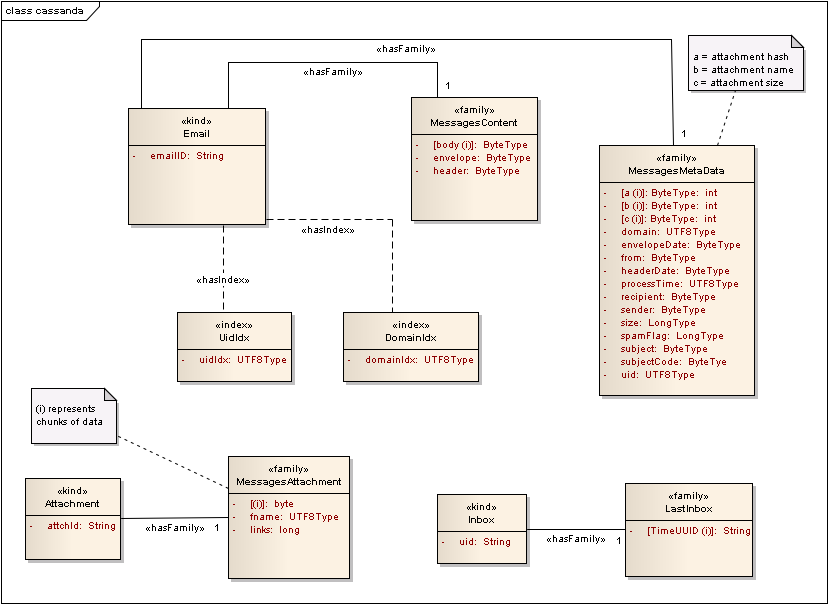
\includegraphics[width=17cm]{./figures/cassandra.png}
 % topologies802154.png: 722x407 pixel, 72dpi, 25.47x14.36 cm, bb=0 0 722 407
 \caption{Databázová schéma}
 \label{fig:Cschema}
\end{figure}

\section{Fultextové vyhľadávanie}

Fultextové vyhľadávanie realizujeme pomocou samostatného NoSQL systému Elasticsearch\footnote{http://elasticsearch.org}. Hlavný index, ktorý obsahuje všetky zaindexované dáta ma názov emailArchive, a delíme ho na dva typy s názvom email a envelope. Schéma týchto typov obsahuje polia poďla, ktorých chceme v emailovom archíve vyhľadávať a jej reprezentáciu zapísanú vo formáte JSON znázorňuje obrázok \ref{fig:ESschema}.

\begin{figure}[h]
\begin{verbatim}
mappingsEmail = {
  "inbox": {"type": "string"},
  "from": {"type": "string"},
  "subject": {"type": "string"},
  "date" :{"type": "date"},
  "messageID" :{"type": "string", "index": "not_analyzed"},
  "attachments":{"type": "string"},
  "size": {"type": "long", "index": "not_analyzed"},
  "body": {"type": "string"}
}   
            
mappingsEnvelope = {
  "sender": {"type": "string"},
  "recipient": {"type": "string"},
  "ip": {"type": "ip"},
  "date": {"type": "date"}
}     
\end{verbatim}
 \caption{JSON schéma pre fultextové vyhľadávanie}
 \label{fig:ESschema}
\end{figure}      


\section{Implementácia}

%Consistent rad - write    W  + R > RF
V programovacom jazyku Python sme implementovali klienta pre zápis dát do databáze Cassandra a ElasticSearch. Jednou z najdoležitejších vlastností týchto klientov je voľba úrovne konzistencie pri zápise. Našou prioritou je integrita dát a od databáze požadujeme silnú konzistenciu. Zvolili sme mód kvóra (ang. Quorum), ktorá zabezpečí zápis dát na N / 2 + 1 replík a klient následne obdrží potvrdenie o úspešnosti zápisu, inak sa zápis zopakuje. Klient, ktorý slúži na čítanie dát z databáze využíva taktiež mód kvóra. Tieto vlastnosti nám zabezpečujú, v prípade použitia faktoru replikácie tri (dáta sa v databázovom systéme nachádzajú trikrát), silnú úroveň konzistencie na strane klienta a databáze. Analýza emailovej správy a jej deduplikácia spotrebúva hlavne CPU zdroje. Moderné procesory obsahuju viacero jadier, tento fakt môžeme využiť pre paralelizované spracúvanie emailov, teda každé jadro CPU bude spracúvať súčasne jednu emailovú správu.

\subsection*{Celery}
Paralelizáciu našej aplikácie sme zabezpečili pomocou využitia asynchrónnej fronty úloh pod názvom Celery\footnote{http://celeryproject.org}, ktorá využíva architektúru distribuovaného predávania správ (ang. distributed message passing). Architektúru znázorňuje obrázok \ref{fig:Celery}. \uv{Pracovníci} (angl. workers) reprezentujú samostatné procesy v našom prípade proces pre analýzu a deduplikáciu emailu, ktoré môžu bežať paralelne. Ako sprostredkovateľ (ang. broker) je použitá aplikácia RabbitMQ\footnote{http://www.rabbitmq.com}, ktorý obdrží od klienta správu a uloží ju do fronty. Správa obsahuje identifikátor emailovej správy, v tomto prípade cestu na lokálnom súborovom systéme k súboru reprezentujúcom email. Táto správa je následne zaslaná ľubovoľnému pracovníkovy (v našom prípade klient kykonávajúci analýzu a deduplikáciu emailu), ktorý ju spracuje. Táto architektúra je plne distribuovaná, dokáže odolávať chybám (napr. v prípade výpadku elektrickej energie, správy nadalej pretrvávajú vo fronte).

%TODO:
\begin{figure}[h]
 \centering
 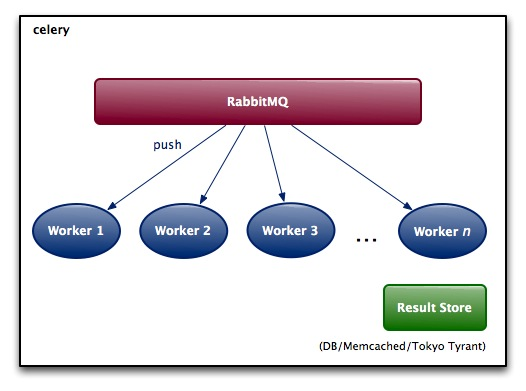
\includegraphics[width=10cm]{./figures/Celery.jpg}
 \caption{Architektúra Celery, Zdroj: [online], http://ask.github.com/celery/getting-started/introduction.html}
 \label{fig:Celery}
\end{figure}



\subsection{Klient}

Proces spracovania nového emailu je znázornený pomocou sekvenčného diagramu na obrázku \ref{fig:Cseq}. Pri príchode nového emailu, ktorý je spracovaný emailovým serverom Qmail, je vytvorená nová úloha pomocou aplikácie Celery. Táto úloha uloží do sprostredkovateľa identifikátor emailu. V prípade, že je v daný okamžik k dispozícií ľubovoľný pracovník, je emailová správa spracovaná pomocou nášho analyzátora a následne zapísaná do databáze Cassandra a fultextového systému Elasticsearch. Na testovacie účely sme nemali k dispozícii reálny dátový tok emailov. Vrstvu reprezentujúcu Qmail sme nahradili modulom, vytvárajúcim nové úlohy prechádzaním lokálneho súborového systému, ktorý obsahoval testovaciu množinu emailový správ.


\begin{figure}[h]
 \centering
 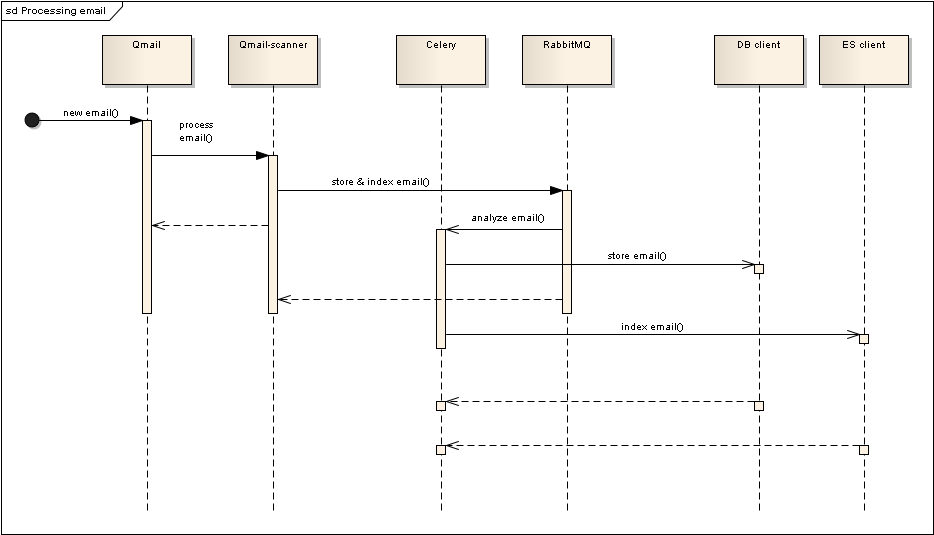
\includegraphics[width=16cm]{./figures/emailProcessing.png}
 % topologies802154.png: 722x407 pixel, 72dpi, 25.47x14.36 cm, bb=0 0 722 407
 \caption{Spracovanie emailu}
 \label{fig:Cseq}
\end{figure}


%Návrh realizácie
%deployment diagram ( oddelene datacentra - na tretej replikacii pocitat MR)ty?

\subsection{Výpočet štatistík}

%TODO PIG = kecy okolo 
% a nepodporuje možnosť definície viackrokového dátového toku \cite{Gates:2009:BHD:1687553.1687568}
Cassandra spolupracuje so systémom Hadoop, čo nám dáva do rúk mocný nástroj na masívne paralelné spracovanie dát pomocou techniky MapReduce. Tvorba aplikácií v tomto frameworku prebieha v Jave, je náročná a okrem toho programový model MapReduce obsahuje viaceo problémov. Model napríklad neobsahuje primitíva na filtrovanie, agregáciu, spájanie dát a je potrebná ich vlastná implementácia. Tieto nedostatky rieši nástroj Pig\cite{} vďaka, ktorému sme boli schopný spracúvať meta dáta uložené v databáze. Obrázok \ref{fig:PigExample} zobrazuje programovú ukážku, ktorá slúži na výpočet veľkosti najvačsieho emailu pre domény, ktorých emaily archivujeme. Pre jednoduchosť sme vynechali časti, ktoré slúžia na načítanie dát z databáze a obsahujú uživateľsky definovanú funkciu v programovacom jazyku Java, ktorá slúži na predprípravu vstupných dát. Podpora uživateľom definovaných funkcií je jednou z ďalších výhod nástroja Pig.

\begin{figure}[h]
\begin{verbatim}
notSpam = FILTER grp BY group.spam == 1;
maxSize = foreach grp {
  size = rows.size;
  generate group, MAX(size);
};
STORE maxSize into 'biggestEmailPerDomainDomain' using PigStorage(',');
\end{verbatim}
 \caption{Programová ukážka v jazyku Pig}
 \label{fig:PigExample}
\end{figure}  



\subsection{Webové rozhranie}
TODO
web IFACE -- pristup koncovych uservo k archivu a diskusia ohladne bezpecnosti - strucny popis django aplikacie.



\section{Overenie návrhu}

Pomocou vyšie popísaného návrhu a implementovaných nástrojov sme overili funkčnosť nami navrhovaného modelu. Vhodná voľba daných verzií u aplikácií Celery a RabbiMQ bola určená počas písania a ladenia aplikácie. Všetky tieto aplikácie sú neustále vo vývoji, to isté platí pre databázu Cassandra a systém Hadoop. Počas písania tejto práce prebehlo viacero rozhovorov s autormi týchto aplikácii. Konkrétne databáza Cassandra na začiatku práce neobsahovala takmer žiadnu ucelenú dokumentáciu, počas začiatkov experimentov sme začínali s verziou 0.7.0. Počas ukončovania tejto práce je aktuálna verzia 0.8.? a medzitým vznikla kvalitná dokumentácia od spoločnosti Datastax\footnote{https://datastax.com}. 

\subsection*{Konfigurácia}
Hardverová konfigurácia bola totožná s konfiguráciou z kapitoly ???. Na šiestich serveroch bola nainštalovaná databáza Cassandra 0.7.3, Hadoop 0.20.2, dvojica serverov obsahovala klientskú aplikáciu a Celery 2.6. V úlohe sprostredkovateľa bola použitá aplikácia RabbitMQ 2.1.1, ktorá bola nainštalovaná na samostatnom serveri.
%TODO-- analyza datasetu HIstogram.. === do analyzy poziadavkov

\subsection*{Overenie integrity dát}
Databázový kluster sme naplnili testovacími dátami obsahujúcimi emaily o objeme 300 GB. Následne sme nasimulovali prípad obnovy dát z archívu, kde sme všetky emaily v náhodnom poradí z databázy načítali, zostavili ich do pôvodného tvaru klientskou aplikáciou a porovnali sme ich odtlačok pomocou hašovacej funkcie MD5 s odtlačkom pôvodných dát. Tento test prebehol bez akejkoľvek chyby. 

\subsection*{Dosiahnuté výsledky}
Doležitým pozorovaním bol fakt, že z celkového objemu emailových správ 300 GB sa po deduplikácií príloh tento objem znížil na 99 GB, teda došlo k 30\% úspore diskovej kapacity. Štruktúry do ktorých sme ukladali dáta pre potrebu štatistík zaberali 0,4\% z celkového objemu dát, čo je zanedbateľná položka.

ES rychlost pre vyhladavanie bola do XY ms.


%Rabbit rychlost

\chapter{Záver}
%kolko deduplikacia
%kolko MB attacch
%mapreduce - PIG
%popis vysledkov
%kolko tvorili indexy














%*****************************************************************************




%\item Zhodnocení splnění cílů DP/BP a  vlastního přínosu práce (při formulaci je třeba vzít v potaz zadání práce).
%\item Diskuse dalšího možného pokračování práce.

%*****************************************************************************
% Seznam literatury je v samostatnem souboru reference.bib. Ten
% upravte dle vlastnich potreb, potom zpracujte (a do textu
% zapracujte) pomoci prikazu bibtex a nasledne pdflatex (nebo
% latex). Druhy z nich alespon 2x, aby se poresily odkazy.

\bibliographystyle{abbrv}
%bibliographystyle{plain}
%\bibliographystyle{psc}
{
%JZ: 11.12.2008 Kdo chce mit v techto ukazkovych odkazech take odkaz na CSTeX:
\def\CS{$\cal C\kern-0.1667em\lower.5ex\hbox{$\cal S$}\kern-0.075em $}
\bibliography{reference}
}

% M. Dušek radi:
%\bibliographystyle{alpha}
% kdy citace ma tvar [AutorRok] (napriklad [Cook97]). Sice to asi neni  podle ceske normy (BTW BibTeX stejne neodpovida ceske norme), ale je to nejprehlednejsi.
% 3.5.2009 JZ polemizuje: BibTeX neobvinujte, napiste a poskytnete nam styl (.bst) splnujici citacni normu CSN/ISO.

%*****************************************************************************
%*****************************************************************************
\appendix


%*****************************************************************************
\chapter{Zoznam použitých skratiek}

\begin{description}
\item[WPAN] Wireless Personal Area Network
\end{description}


%*****************************************************************************
\chapter{Inštalačná a užívateľská príručka}

\subsection{Inštalácia simulátoru OMNeT++ pre platformu Linux}
\begin{enumerate}
 \item Stiahnutie archívu obsahujúceho zdrojový kód zo stránok \\
 \url{http://www.omnetpp.org/omnetpp}
 \item Prekopírovanie archívu do adresára /usr/local/
 \item Rozbalenie archívu pomocou príkazu tar zxvf omnetpp-4.0.src.tgz
 \item Do užívateľského profilu .bash\_profile alebo .profile pridáme riadok \\
  export PATH=\$PATH:/usr/local/omnetpp-4.0/bin
  \item Je potreba zabezpečiť prítomnosť následujúcich balíkov v systéme 
    \begin{tabbing}
    sudo apt-get install \= build-essential gcc g++ bison flex perl tcl8.4 tcl8.4-dev \\
                       \> tk8.4 tk8.4-dev blt blt-dev libxml2 libxml2-dev \\
                       \> zlib1g zlib1g-dev libx11-dev
    \end{tabbing}    
 \item Prevedieme následujúce príkazy: \\
   cd /usr/local/ometpp-4.0 \\
   ./configure \\
   ./make
 \item Spustenie OMNeT++ s IDE pomocou príkazu omnetpp 
\end{enumerate}

\subsection{Inštalácia mnou modifikovaného Mobility Frameworku}
\begin{enumerate}
 \item Stiahnutie súborov Mobility frameworku z svn http://my-svn.assembla.com/svn/mframework/, poprípade prekopírovanie adresára mf2o4 z priloženého CD do adresára /usr/local/
 \item Import MF do aplikácie OMNeT++
  \begin{enumerate}
   \item Po spustení aplikácie Omnet, klikneme na oblasť \uv{Project explorer}, pravým tlačítkom a zvolíme položku \uv{Import...}
   \item Zvolíme \uv{General->Existing project into Workspace}
   \item V položke \uv{Select root directory}, zvolíme cestu k adresáru mf2o4, tj. /usr/local/mf2o4
   \item Pomocou CTRL+B, preložíme zdrojové súbory
  \end{enumerate}  
\end{enumerate}

\subsection{Práca s modelom IEEE 802.15.4}
Vo vývojom prostredí Omnetu si otvoríme v oblasti \uv{Project explorer} adresárovú štruktúru mf2o4, kde si následne otvoríme adresár networks a v ňom adresár ieee802.15.4. V tomto adresári sa nachádzajú aj xml súbory popisujúce antény. Otvoríme si súbor omnetpp.ini, tento súbor je hlavným konfiguračným súborom modelu simulácie. Zahrnul som do neho ukážkové nastavenia viacerých modelov, ktoré som simuloval. Samotná simulácia sa potom spustí otvorením súboru omnetpp.ini a následným kliknutím na tlačítko \uv{Run} z menu aplikácie.

%*****************************************************************************
\chapter{Obsah priloženého CD}

Následujúci obrázok \ref{fig:zoznamCD} zobrazuje štruktúru priloženého CD.

\begin{figure}[h]
\begin{center}
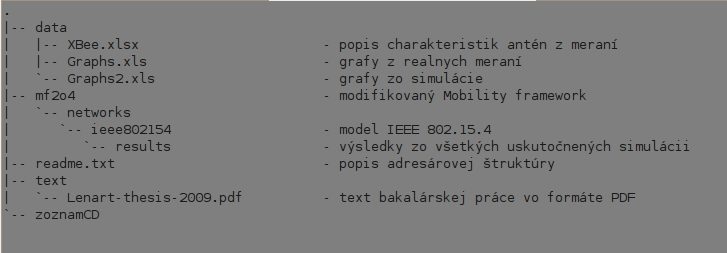
\includegraphics[width=14cm]{./figures/zoznamCD.png}
\caption{Výpis priloženého CD}
\label{fig:zoznamCD}
\end{center}
\end{figure}

\end{document}
